%% This is file `elsarticle-template-3-num.tex',
%%
%% Copyright 2009 Elsevier Ltd
%%
%% This file is part of the 'Elsarticle Bundle'.
%% ---------------------------------------------
%%
%% It may be distributed under the conditions of the LaTeX Project Public
%% License, either version 1.2 of this license or (at your option) any
%% later version.  The latest version of this license is in
%%    http://www.latex-project.org/lppl.txt
%% and version 1.2 or later is part of all distributions of LaTeX
%% version 1999/12/01 or later.
%%
%% The list of all files belonging to the 'Elsarticle Bundle' is
%% given in the file `manifest.txt'.
%%
%% Template article for Elsevier's document class `elsarticle'
%% with numbered style bibliographic references
%%
%% $Id: elsarticle-template-3-num.tex 165 2009-10-08 07:58:10Z rishi $
%% $URL: http://lenova.river-valley.com/svn/elsbst/trunk/elsarticle-template-3-num.tex $
%%
%\documentclass[preprint,12pt]{elsarticle}

%% Use the option review to obtain double line spacing
%% \documentclass[preprint,review,12pt]{elsarticle}

%% Use the options 1p,twocolumn; 3p; 3p,twocolumn; 5p; or 5p,twocolumn
%% for a journal layout:
%% \documentclass[final,1p,times]{elsarticle}
%% \documentclass[final,1p,times,twocolumn]{elsarticle}
%% \documentclass[final,3p,times]{elsarticle}
\documentclass[preprint,3p,times,twocolumn]{elsarticle}
%% \documentclass[final,5p,times]{elsarticle}
%% \documentclass[final,5p,times,twocolumn]{elsarticle}

%% if you use PostScript figures in your article
%% use the graphics package for simple commands
%% \usepackage{graphics}
%% or use the graphicx package for more complicated commands
%% \usepackage{graphicx}
%% or use the epsfig package if you prefer to use the old commands
%% \usepackage{epsfig}

%% The amssymb package provides various useful mathematical symbols
\usepackage{amssymb}
\usepackage{amsmath}
%% The amsthm package provides extended theorem environments
%% \usepackage{amsthm}

%% The numcompress package shorten the last page in references.
%% `nodots' option removes dots from firstnames in references.
% \usepackage[nodots]{numcompress}

%% The lineno packages adds line numbers. Start line numbering with
%% \begin{linenumbers}, end it with \end{linenumbers}. Or switch it on
%% for the whole article with \linenumbers after \end{frontmatter}.
\usepackage{lineno}
\usepackage{xcolor}
\usepackage{subfigure}
\usepackage{multirow}
%% Avoids linenumbers to collide with text for 5p format:
\setlength\linenumbersep{3pt}

%% natbib.sty is loaded by default. However, natbib options can be
%% provided with \biboptions{...} command. Following options are
%% valid:

%%   round  -  round parentheses are used (default)
%%   square -  square brackets are used   [option]
%%   curly  -  curly braces are used      {option}
%%   angle  -  angle brackets are used    <option>
%%   semicolon  -  multiple citations separated by semi-colon
%%   colon  - same as semicolon, an earlier confusion
%%   comma  -  separated by comma
%%   numbers-  selects numerical citations
%%   super  -  numerical citations as superscripts
%%   sort   -  sorts multiple citations according to order in ref. list
%%   sort&compress   -  like sort, but also compresses numerical citations
%%   compress - compresses without sorting
%%
%% \biboptions{comma,round}

% \biboptions{}


\journal{Computers \& Graphics}

\begin{document}

\begin{frontmatter}

%% Title, authors and addresses

%% use the tnoteref command within \title for footnotes;
%% use the tnotetext command for the associated footnote;
%% use the fnref command within \author or \address for footnotes;
%% use the fntext command for the associated footnote;
%% use the corref command within \author for corresponding author footnotes;
%% use the cortext command for the associated footnote;
%% use the ead command for the email address,
%% and the form \ead[url] for the home page:
%%
%% \title{Title\tnoteref{label1}}
%% \tnotetext[label1]{}
%% \author{Name\corref{cor1}\fnref{label2}}
%% \ead{email address}
%% \ead[url]{home page}
%% \fntext[label2]{}
%% \cortext[cor1]{}
%% \address{Address\fnref{label3}}
%% \fntext[label3]{}

\title{Efficient 3D Reconstruction of Vessels from Multi-views of X-Ray Angiography}

%% use optional labels to link authors explicitly to addresses:
%% \author[label1,label2]{<author name>}
%% \address[label1]{<address>}
%% \address[label2]{<address>}

\author{Anonymous submission}

\address{}

\begin{abstract}
%% Text of abstract
In this paper, we present an efficient 3D vessels reconstruction algorithm
based on multi-views of X-ray Angiography assisting interventional surgery.
First, we extract the vascular-like structures from the image sequences
using a geometrical analysis of multi-scale Hessian matrix eigen-system and
use the fast marching method to extract the skeleton of the structure, from
which we derive the vascular topological configurations. Second, we regard
the 3D space as a Markov Random Field and formulate the reconstruction
problem as an energy minimization problem with consistent, continuous and
topological constraints to coarsely register and reconstruct the 3D vessels.
Third, we refine the reconstructed vessels to register and reconstruct the
3D vessels accurately. We demonstrate our system in coronary arteries
reconstruction for percutaneous coronary intervention surgery to help
doctors learn about the configurations of the coronary arteries of specific
patient during operation. We envision that our system will be used for
clinic treatment to advance vessel reconstruction for diagnosis and therapy
in the near future.

\end{abstract}

\begin{keyword}
%% keywords here, in the form: keyword \sep keyword
X-Ray angiography \sep 3D reconstruction \sep Multi-scale retinex \sep Belief propagation
%% MSC codes here, in the form: \MSC code \sep code
%% or \MSC[2008] code \sep code (2000 is the default)
\end{keyword}

\end{frontmatter}

%%
%% Start line numbering here if you want
%%
\linenumbers

%% main text
\section{Introduction}\label{sec:introduction}
Intraoperative X-Ray is essential during some surgeries, such as
percutaneous coronary intervention. The 2D X-Ray images not only lose
a significant amount of 3D information of the coronary arteries, but
also suffer from the viewing angle dependence, magnification factor,
overlapping and the blurring between vessels, backgrounds and other
tissues and organs.

Great efforts have been done on 3D reconstruction of coronary arteries
to overcome the shortcomings of 2D images. But there are also some
problems existing in current methods. First, the absence of image
enhancement procedures may lead to disappearance of some tiny details
because of the low contrast and blurring of angiograms. Second, the
vessel skeleton extraction methods are not accurate and may acquire
discontinuous or unsmooth results. Third, accurate reconstructions
need five or more views of angiograms with exact angle requirements,
which is hard to operate for clinical use. Fourth, current 3D
reconstruction methods mostly rely on the registrations between image
pairs, which are hard to add constrain conditions such as consistency
and continuity.

To overcome these shortcomings, we present an efficient vessel
reconstruction system from multiple X-Ray views. The pipeline is shown
in Figure \ref{fig:procedure}. First, we apply the multi-scale retinex
method to enhance the contrast of the angiogram. Second, we implement
a CUDA edition of Hessian matrix based vessel filter with hysteresis
thresholding to get the preprocessing results. Third, we perform the
fast-marching method using second order derivatives and cross neighbor
templates to extract the accurate centerline of the
vascular-structure. Finally, 3D reconstruction with local constraints
and space consistencies is formulated as an energy minimization
problem and solved using belief propagation. All these lead to a fast
reconstruction result of the data and promise accuracy and efficiency
which can give the doctor a good sense of coronary artery 3D space
structures. The contributions of the paper are:

(1) We combine the MSR enhanced images which are mostly over extracted
with line segments tracking methods to obtain more detailed vessels
from blurry angiograms.

(2) We divide the spaces between the X-Ray iso-center and the detector
into slices in which we sample the 3D space points and project them to
the image space considering consistency and continuity with their
neighbors, overcoming the lack of constraints for typical
registrations.

(3) We formulate the 3D reconstruction as a global energy
optimization problem and solve it by using belief propagation.


\begin{figure*}
  \centering
  % Requires \usepackage{graphicx}
  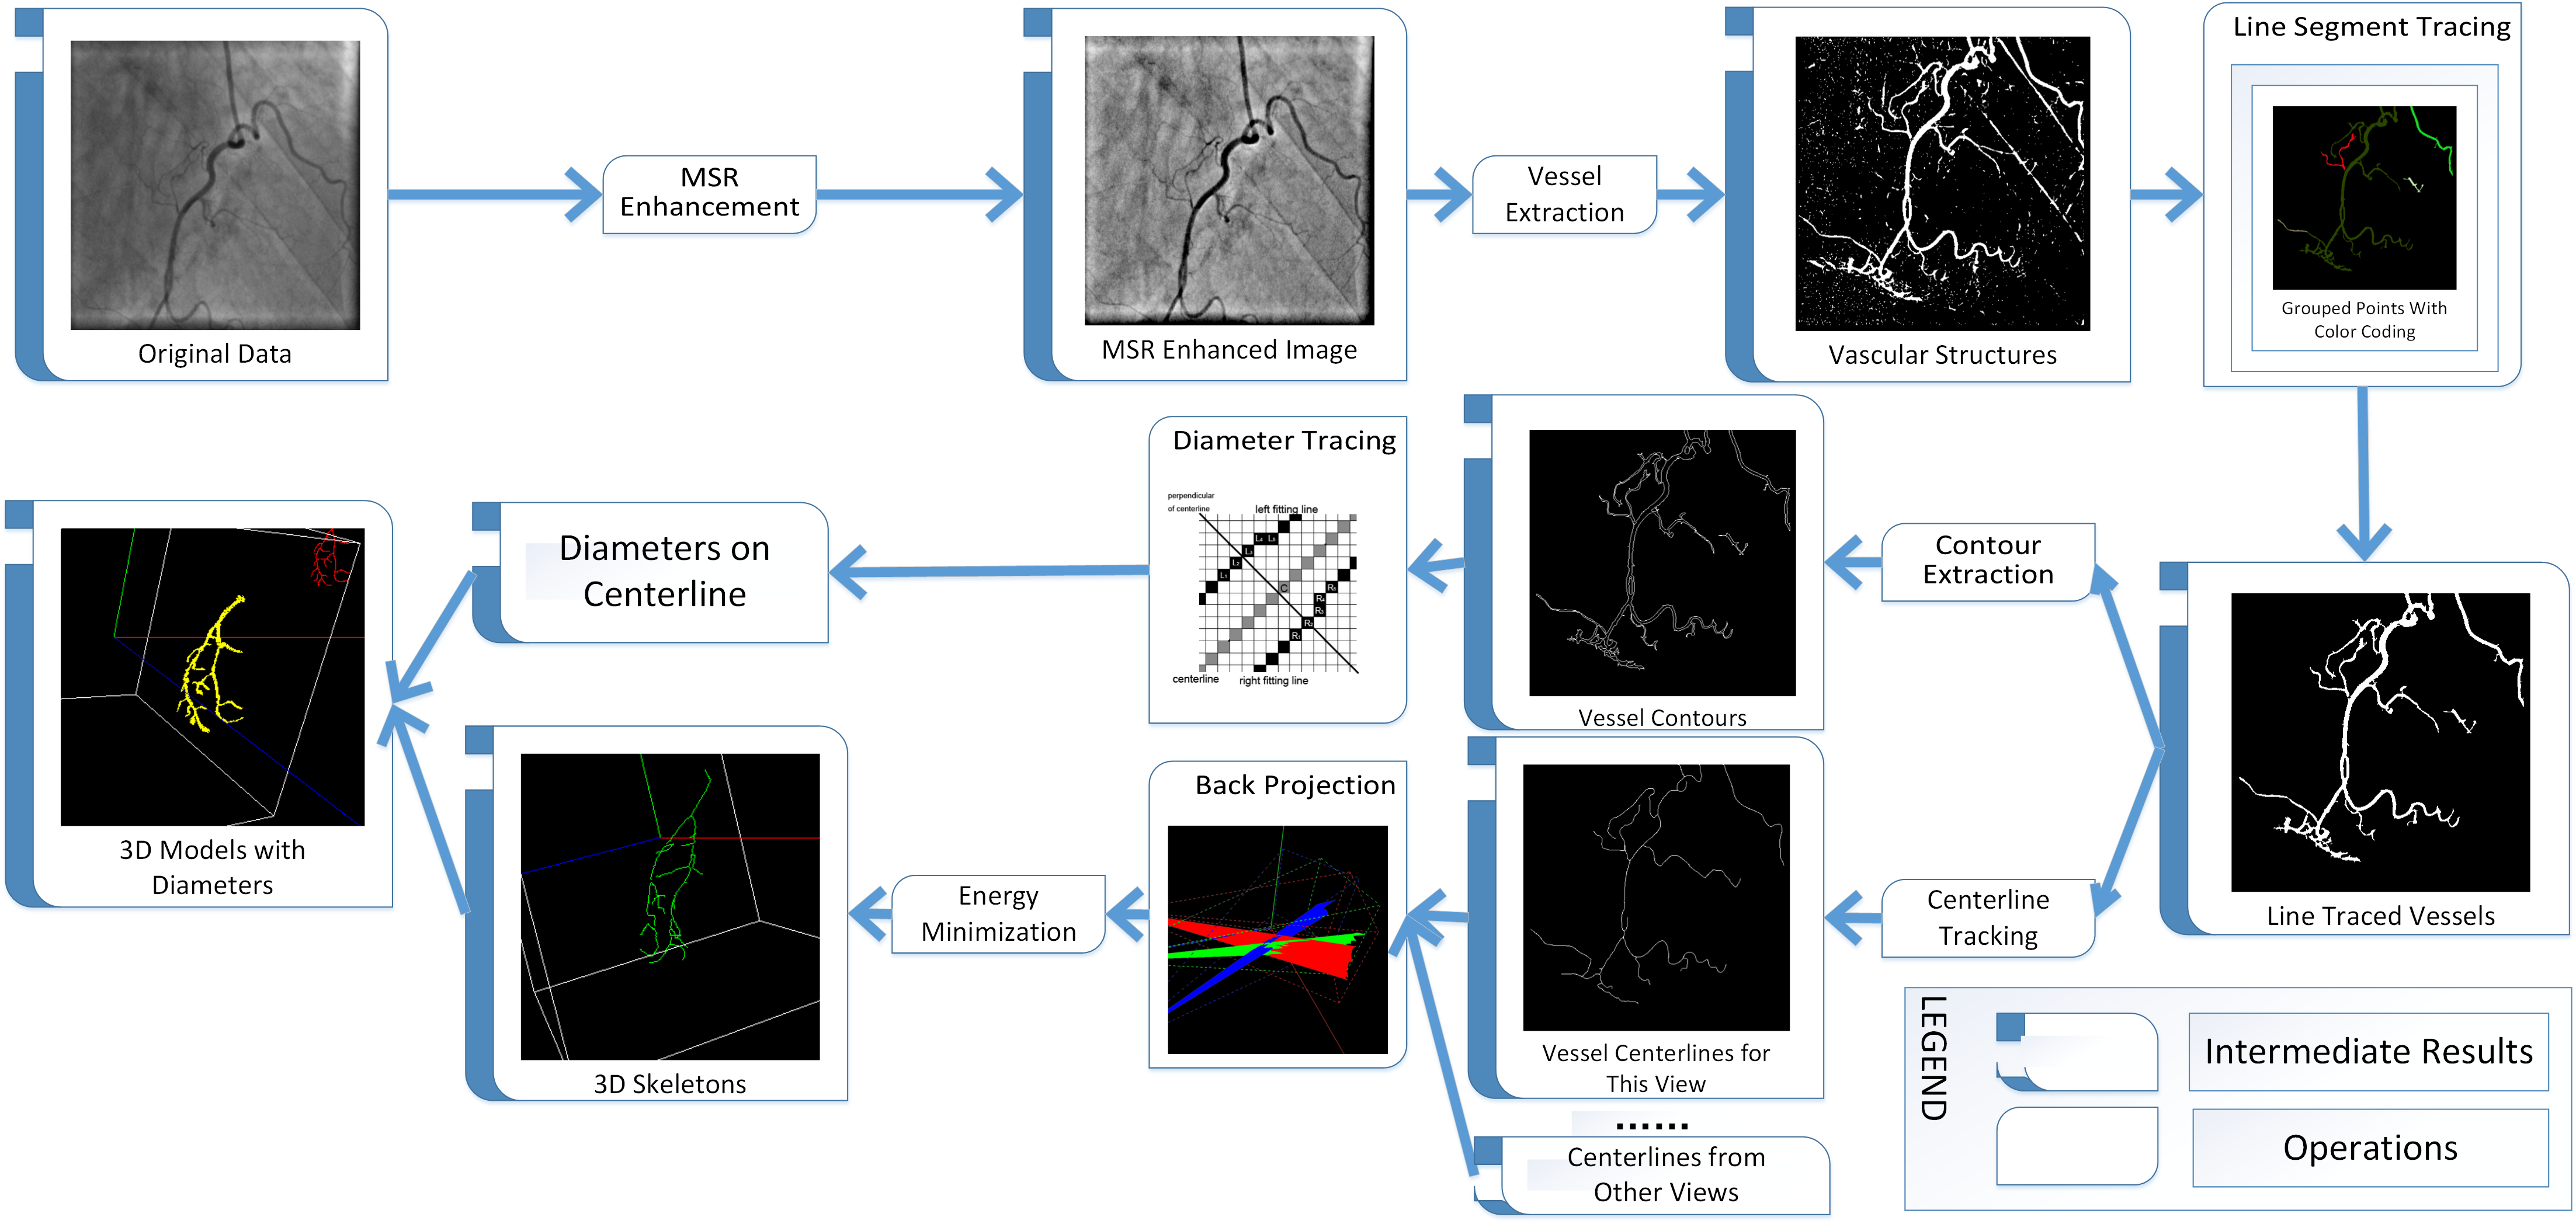
\includegraphics[width=6.0in]{procedure.png}\\
  \caption{Work Pipelines}\label{fig:procedure}
\end{figure*}


\section{Related Work}\label{sec:relatedwork}

Our work relates to vessel extraction from image and vessel
reconstruction etc. We briefly review them in the following
categories.

\subsection*{Vessel Extraction}
Hoover et al.~\cite{Hoover} use a mathematical filter to entails a
broad range of vessel enhancement and Li et al.~\cite{Li} do this
using a non-linear filter. Frangi et al.~\cite{Frangi} use the eigen
values of Hessian matrix to extract the tube-like structures from the
X-Ray images. Condurache et al.~\cite{Condurache} use this method
while adding a hysteresis thresholding method to purify the extracted
data.

\subsection*{Centerline Extraction}
Centerline extraction consists of six kinds of techniques: pattern
recognition techniques, deformable model based techniques
\cite{Deformable1}\cite{Deformable2}\cite{Deformable3}, tracking-based
techniques \cite{Tracking1}\cite{Tracking2}\cite{Tracking3} \cite{Tracking4}
\cite{Tracking5}, artificial intelligence-based techniques, neural
network-based techniques and miscellaneous tube-like object detection
techniques. Each one contains many sub-types such as multi-scale approaches,
mathematical morphology approaches. Readers please refer to~\cite{Kirbas}
for an overview of the centerline extraction technologies.

\subsection*{3D Reconstruction}

As with 3D reconstruction, Wellnhofer et al.~\cite{Wellnhofer} and Messanger
et al.~\cite{Messenger} evaluate that 3D reconstructions of coronary
arteries from 2D X-Ray image sequences permit accurate results of the real
data. The two types of the X-Ray machine lead to two slightly different ways
of 3D reconstruction. The biplane system takes two (mostly) synchronized
projection of the coronary arteries~\cite{Wellnhofer}\cite{Messenger}.
Meanwhile the mono-plane (single-plane) system~\cite{Gollapudi} can just
take one view at the same time, therefore selection of asynchronous images
from multiple views is needed. However, using only two 2D projections to
reconstruct the complex 3D topology of coronary artery is often not
sufficient. Movassaghi et al.~\cite{Movassaghi} uses multiple projections
for realistic vessel lumen simulations, but only uses two for 3D centerline
reconstruction. Sprague et al.~\cite{Sprague} utilizes the benefits of three
projections experimentally. Hansis et al.~\cite{Hansis} has used multiple
projections from a single rotational X-Ray angiography to reconstruct the 3D
centerline and the topology. Nguyen et al.~\cite{Nguyen} propose a method
based on motion and multiple views using a single-plane imaging system. They
only consider the rotation and scaling of the heart motion but rigorously
the heart motion during contraction and relaxation consists of five
movements: translation, rotation, wringing, accordion-like motion and
movement towards the center of the ventricular chamber~\cite{Marcus}.
Therefore, a simple motion can not generally describe the heart cardiac
cycle.

Other routines such as knowledged-based or rule-based have been
proposed for 3D reconstruction using the vascular network
model~\cite{rule_based1} \cite{rule_based2}. Since their rules or
knowledge are designed for specific conditions, it is not easy to
generalize these kinds of methods to process artery data.

In~\cite{opti_est1}\cite{opti_est2}\cite{opti_est3}, optimal
estimation are investigated with a two-step approach based on
maximum-likelihood and minimum-variance estimation. They use a linear
algorithm to compute the preliminary estimates as the initial
estimates for the process of optimal estimation. Due to the huge
computation, none of the existing techniques have been used in
clinical therapy.

\subsection*{Other Focuses}

Another focus on 3D reconstruction is on the elimination or
minimization of foreshortening and overlap of the coronary arteries
which is a prerequisite for an accurate quantitative coronary analysis
such as the vessel lengths and aneurysms. In~\cite{opti_view1},
they focus on the minimization of vessel foreshortening relative to
a single arterial segment. Sato et al.~\cite{opti_view2} and
Finet et al.~\cite{opti_view3} introduce an
optimal view selection method considering both foreshortening and
vessel overlap. Chen et al.~\cite{James_Chen} use bifurcation points
and the vessel directional vectors of bifurcations to register between image
pairs. Meanwhile, they also proposed a method of selecting
the minimized foreshortening views. But, it depends on bifurcations
overmuch and requires at least five pairs of bifurcations to ensure
accurate transformation. Also, their work is time consuming with a
whole procedure of ten minutes.


\section{Methods}\label{sec:methods}
\subsection{Data Acquisition and Preprocessing}

\subsubsection{Data Acquisition}
For all procedures, we use two types of data. One is the synthetic data from our simulation
system described in Figure \ref{fig:simu_plaform} with vessel trees' ground truth known.
The other one is the real data from the clinical angiogram.

\begin{figure}
  \centering
  % Requires \usepackage{graphicx}
  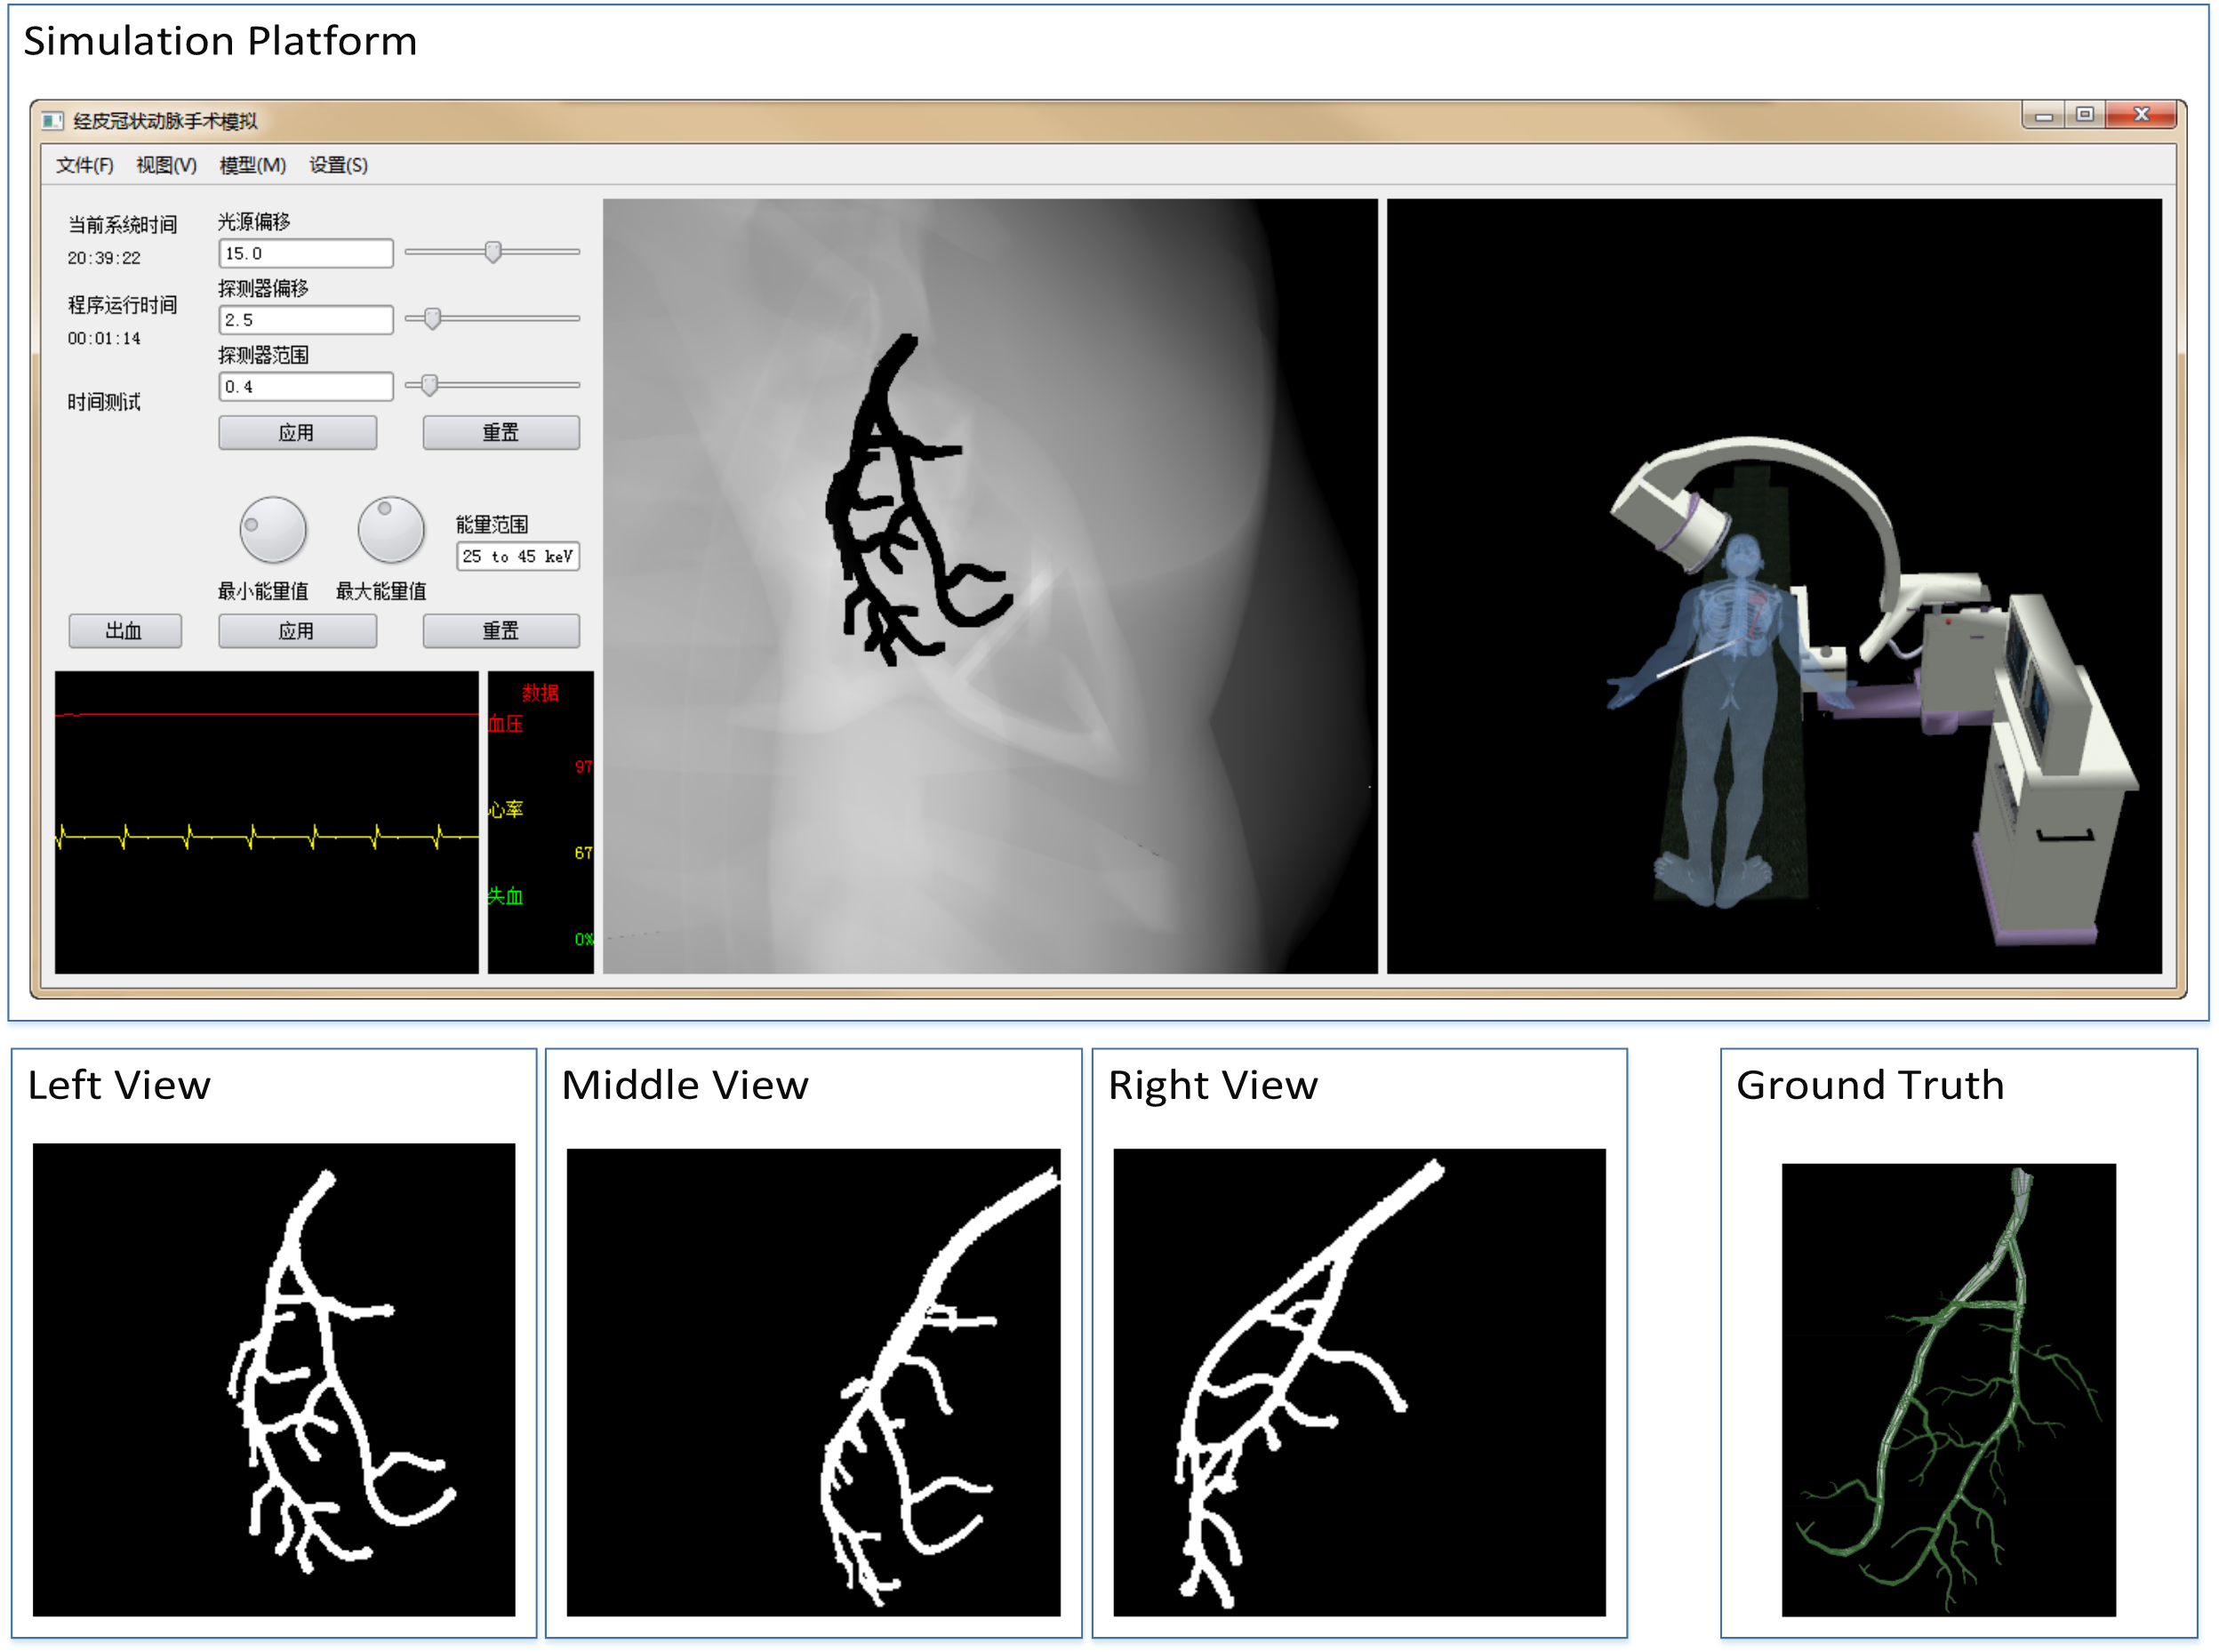
\includegraphics[width=3.0in]{simu_platform_with_data.png}
  \caption{Our Simulation Platform}
  \label{fig:simu_plaform}
\end{figure}

For simulation data, we use three different views respectively at RAO 50, LAO 50, LAO 0,
while at the same CRA angle. For real data, we use LAO 2, CRA 29 as the middle view, and
LAO 32, CRA 27 as the left reference view, and RAO 25 CRA 29 as the right view. All the
sequences of the views consist at least 50 images with the pixel resolution of 512 $\times$ 512.
We select one image from each view at the mostly the same cardiac cycle and use them to
reconstruct the vessels.


%%
%%comment: In this subsection. Too many contents are others' work, but few are yours.
%%
\subsubsection{Multiscale Retinex Image Enhancement}
The original angiograms acquired from the X-Ray machine have many
shortcomings such as the low image contrast, the low lumen with the
wide dynamic range. Current methods for X-Ray angiograms enhancement
such as gain/offset fix, histogram equalization can only work well for
specific angiograms. Take histogram equalization for example, it can
only handle images with one single apex, while for double or several
apexes, satisfactory results can not be achieved. In our approach, we
apply an enhancement of radiography based on Multiscale Retinex.

Land et al.~\cite{Land_Retinex} first proposed the Retinex as a model
for human perception of brightness and color and formulates the ideal
images as

\begin{equation}\label{retinex}
f(x,y)=r(x,y)\times i(x,y)
\end{equation}

where $i(x,y)$ is the environment brightness function which describes
the brightness of the surroundings, while the $r(x,y)$ is the scene
reflection function which describes the ability of the scene to
reflect itself. Jobson et al.~\cite{JOBSON_Retinex} defined the single
retinex algorithm which can be described as

\begin{equation}
R(x,y) = \log I(x,y)- \log [F(x,y) \ast I(x,y)]
\end{equation}

where $R(x,y)$ is the output image, $I(x,y)$ is the input image,
$\ast$ stands for convolution, $\log$ is the natural log, $F(x,y)$ is
the environment function. Moore \cite{MOORE_Retinex} proposed to use
the

\begin{equation}
F(x,y)=exp(-r/c)
\end{equation}

A better approach for this function is the Hurlbert's \cite{lighting_equotion}
work, they define $F(x,y)$ as

\begin{equation}
F(x,y) = Kexp(-(x^2+y^2)/\sigma^2)
\end{equation}

where $\sigma$ is the standard deviation of gaussian function which
controls the detail preservation, K should afford

\begin{equation}
\iint f(x,y)\mathrm{d}x\mathrm{d}y = 1
\end{equation}

Single Retinex can not achieve good results both on color consistency
and dynamic range compression. We use the method based on Multiscale Retinex(MSR)
which can be described as

\begin{equation}
R_{i} = \sum_{k=1}^{K} W_{k}(\log I_{i}(x,y) - \log[F_{k}(x,y) \ast I_{i}(x,y)])
\end{equation}

where $i$ stands for the $ith$ channel, $K$ stands for the channel
number, $W_{k}$ and $F_{k}$ are the weight coefficients. After MSR, we
use the gain/offset method to fix the negative values of the image

\begin{equation}
R_{o}(x,y)=G \times R_{i}(x,y) + offset
\end{equation}

\begin{equation}
R(x,y)=255 \times \frac{R_{o}(x,y)-r_{min}}{r_{max}-r_{min}}
\end{equation}

where $R_{i}(x,y)$ and $R_{o}(x,y)$ are the image input and output,
$R(x,y)$ is the final grey image.

In our approach, we use four different Gaussian filter coeffients
under four different deviations were calculated. Then we apply a
convolution between the original images and the Gaussian filters and
get a weighted average result of the four different filters. After all
these, the X-Ray angiograms are obviously enhanced with higher
contrast and low dynamic ranges shown in Figure
\ref{fig:enhanced_image}.

\begin{figure}
  \centering
  % Requires \usepackage{graphicx}
  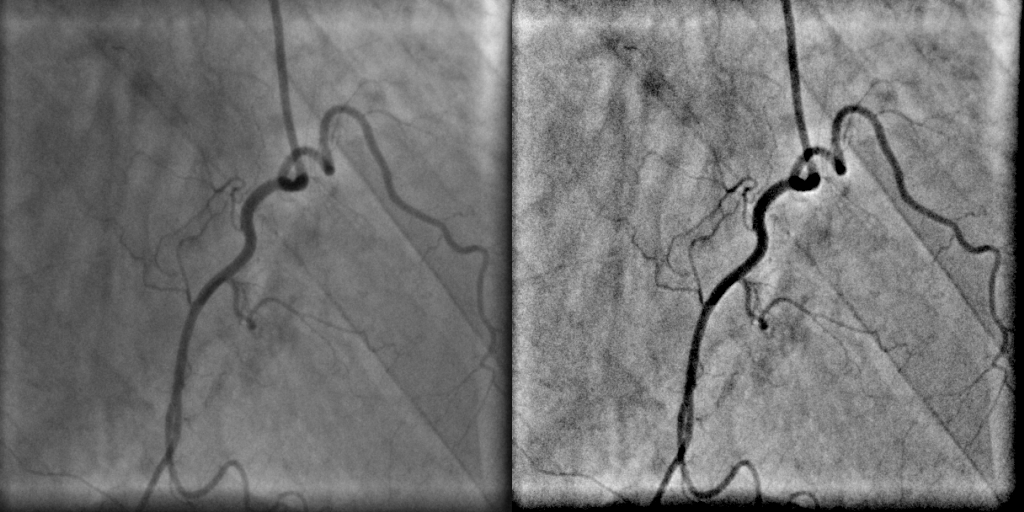
\includegraphics[width=3.0in]{msr_cmp.png}
  \caption{Left: Original Image, Right: Enhanced Image}
  \label{fig:enhanced_image}
\end{figure}



\subsection{Vessel Extraction}
\subsubsection{Vessel extraction based on Hessian matrix}
For vessel extraction on X-Ray angiograms, vessels are often hard to be
sensed due to the low intensity contrast as well as their soft issues. Even
for fine vascular structures, this problem is severe. The major challenge
relies on how to enhance or extract the vascular structure with the
avascular as less as possible.

After achieving the high-contrast images preprocessed by MSR, we use
the approach proposed by \cite{Frangi}
It relies on a multiscale Hessian matrix that enhances the vascular
structures.


%%
%% Those contents can be simplfied
%%
Hessian matrix considers the local features of the vessels.  A common
approach to analyze the local features of a 2D/3D image is to consider
the Taylor expansion in the neighborhood of a point $x_{0}$

\begin{equation}
\label{Taylor}
I(x_{0} + \Delta x) \approx I(x_{0}) + \Delta {x^T} \nabla {I(x_{0})} + \Delta {x^T} H(x_{0}) \Delta x
\end{equation}

where $\nabla I$ is the gradient vector and $H$ donates the Hessian
matrix- which is the second-order partial derivatives of $I$

\begin{equation}
\label{Hessian}
H =
\left(
  \begin{array}{cc}
    I_{xx} & I_{xy}\\
    I_{yx} & I_{yy} \\
  \end{array}
\right)
\end{equation}

For a given scale $\sigma$, the image I is first convoluted with a 2D
Gaussian filter $G_{\sigma}$. The convoluted image can be explained by
$I_{\sigma} = I * G_{\sigma}$. The Hessian matrix of the convoluted
image can be computed by

\begin{equation}\label{Hessian sigma}
HI_{\sigma} =
\left(
  \begin{array}{cc}
    {\frac{\partial^2 I_{\sigma} }{\partial x^2}} & {\frac{\partial^2 I_{\sigma} }{\partial y \partial x}}\\
    {\frac{\partial^2 I_{\sigma} }{\partial x \partial y}} & {\frac{\partial^2 I_{\sigma} }{\partial y^2}} \\
  \end{array}
\right)
\end{equation}

The eigenvalues and eigenvectors of the Hessian can be used to extract
the features of the local structures. The direction of the potential
locally rectilinear structure can be calculated by

\begin{equation}\label{localdirection}
\tan (2D_{\sigma}) = 2 {\frac{\partial^2 I_{\sigma} }{\partial y \partial x}} ({\frac{\partial^2 I_{\sigma} }{\partial x^2}} - {\frac{\partial^2 I_{\sigma} }{\partial y^2}})
\end{equation}

For coronary arteries, their sizes are varied and particularly tiny. In our
experiments, we use the interval [0.3 3] with the step 0.3 to get ten
representations of the original images. Then, for every pixel on the image,
we calculate the second-order derivatives to build the Hessian matrix $H$.
Next, before eigenvalues decomposition, we normalize the Hessian matrix
which is divided by $\sigma^{2}$. After the normalization, we decompose the
Hessian matrix into its corresponding eigenvalues $\lambda_{1},
\lambda_{2}$, here we assume $\vert \lambda_{2} \vert \ll \vert \lambda_{1}
\vert $. According to \cite{Frangi}, we define parameters by

\begin{equation}
\label{Rb}
R_{b} = \frac{\lambda_{2}}{\lambda_{1}}
\end{equation}

which attains its maximum for a blob-like structure and is zero whenever
$\lambda_{2} \approx 0$, or $\lambda_{1}$ and $\lambda_{2}$ tend to vanish.

\begin{equation}
\label{Rb}
S^{2} = {\lambda_{1}}^2 + {\lambda_{2}}^2
\end{equation}

which is used to distinguish plate-like(non-zero) and line-like (zero)
structures. Finally, we get the equation specifying the possibility of
a pixel being one part of vessel structures

\begin{equation}
\label{v0s}
\upsilon_{\sigma}(s)=
\left\{
  \begin{array}{ll}
    0, & \hbox{if $\lambda_{1}<0$,} \\
    exp(-\frac{R_{b}^2}{2\beta^2})(1-exp(-\frac{S^2}{2c^2})), & \hbox{else}
  \end{array}
\right.
\end{equation}

where $\beta$ and $c$ are parameters that control the sensitivity and
continuity of the filter.

Finally, having performed the same process on all the other scales,
the scale with maxima $\upsilon_{\sigma}$ is selected and the
corresponding value is recorded. This value can be regarded as the
possibility of the vascular structures' occurence at this position. We
initialize a new image with the same size as the original image using
Hysteresis Thresholding. The pixel values of the image are the
corresponding values of the recorded values ranging from 0 to 1. The
extraction result are shown in Figure \ref{fig:possibilityimage}.

\begin{figure}
  \centering
  % Requires \usepackage{graphicx}
  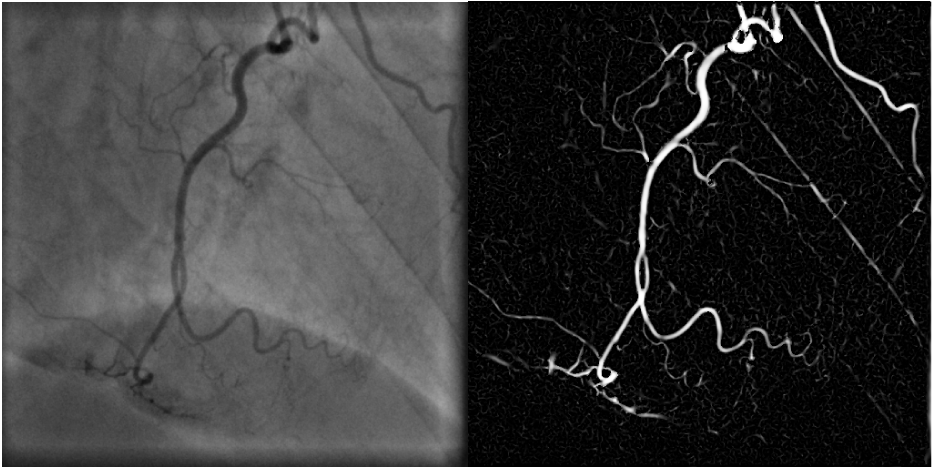
\includegraphics[width=3.0in]{possibilityimage.png}\\
  \caption{Possibility Image}\label{fig:possibilityimage}
\end{figure}

After having got the possibility image, we initialize another new
binary image for calculating centerlines. The pixels where the
extraction values are greater than zero are white while the others are
black. We compute the connectivity of the whole image using a cross
template so that line segments whose length are smaller than a typical
value are regarded as noise as well as many noisy points produced by
enhancement during MSR. After all these steps, we can reduce
over-extraction and noise as much as possible. The tracking result is
shown in Figure \ref{fig:lineseg_trace}.
\begin{figure}
  \centering
  % Requires \usepackage{graphicx}
  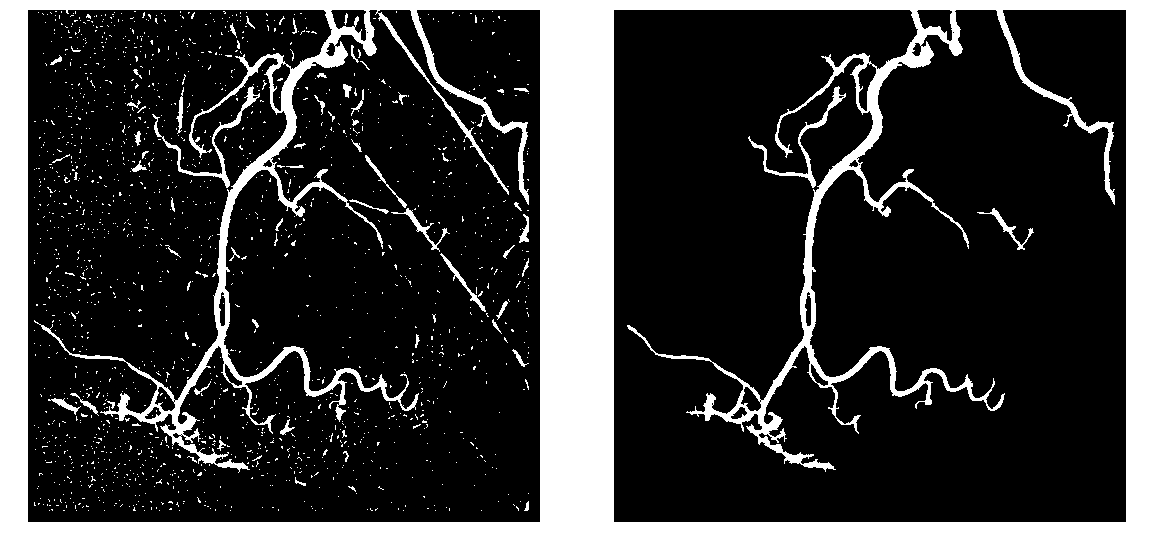
\includegraphics[width=3.0in]{lineseg_trace.png}\\
  \caption{Line Segment Trace Image}\label{fig:lineseg_trace}
\end{figure}

\subsubsection{Hysteresis-like Thresholding}
Hysteresis thresholding is to discard obvious non-vascular structures from
the result images while retaining the definite values. We use a histogram of
the image grey values to compute the quantiles of them as the basis of
thresholds. The low threshold is chosen low enough to obtain a slightly over
detection.


\subsection{Centerline Tracking}
After getting the binary images of the vascular structures, we apply
the centerline extraction method using fast marching based on Hassouna
\cite{Hassouna}'s and Jakob \cite{Jakob}'s  work. They use fast
marching method to obtain an accurate solution of Eikonal equation
known as

$$|\nabla T| F = 1 , \; s.t.\; T(\Gamma_{0})=0$$

where  $\Gamma$ stands for the closed interface that separates one region
from another. Hassouna et al.~\cite{Hassouna} proposed an improved version
of the fast marching method with high accuracy called multistencils fast
marching(MSFM). By solving the Eikonal Equation at each point under several
stencils which cover 8 neighbours in 2D space and 26 in 3D space and picking
up the one which satisfies the upwind condition most, they can achieve
better accuracy. For stencils not aligned with the natural coordinate
system, Eikonal equation is derived using directional derivatives and solved
using higher finite difference schemes.

Our approach is based on Jakob \cite{Jakob}'s  work. The 2D binary
image points can be divided into \textit{frozen} pixels which we
compute distances at their neighbours and \textit{narrow band} pixels.
For each iteration, the \textit{narrow band} pixels having the
smallest distance value is frozen and distances are computed from its
neighbours. Progressively, the \textit{narrow band} pixels propagate
from the initial condition and the freezing pixels follow them along,
finally, when all points are frozen, the method vanishes. During the
procedure, we use the method proposed as Hassouna \cite{Hassouna} to
compute the distances and implement a custom unsorted binary tree
which performs like a normal binary sorted tree to select the minimum
distance in every MSFM iteration.

During the centerline tracking, every point in each line is tracked and the
bifurcations are recorded, finally we can get a vessel centerline tree
including all bifurcations as shown in Figure \ref{fig:centerline}. The left
image is the binary image representing the centerlines of the vessels, the
right is the original image with colored centerlines. Each red cross
represents one bifurcation and each color represents one single centerline.

\begin{figure}
  \centering
  % Requires \usepackage{graphicx}
  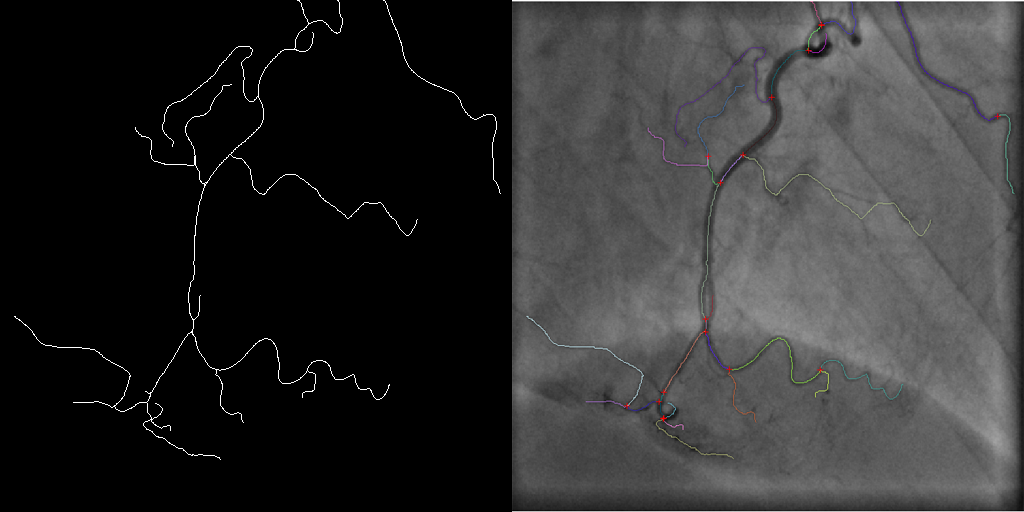
\includegraphics[width=3.0in]{centerline.png}\\
  \caption{Binary and Colored Centerlines}\label{fig:centerline}
\end{figure}


\subsection{Vascular Diameter Extraction}
The vessel diameter is an important indicator for many vascular diseases
from the X-Ray angiogram and the precise estimation of vascular centerlines
and widths is very important for the quantitative and visualized diagnosis
of blood vessel disease. Currently the diagnosis of the vessel from the
angiograms mainly depends on doctors' naked eyes. The diagnosis results are
much affected by human factors and lead to coarse objectivity and low
accuracy.

In our approach, we combine the centerlines and the extracted vascular
structures and use the centerlines as sample bases for diameter computation.
Due to the discreteness of extracted results,  we propose a method based on
line fitting to obtain continuous diameters shown in Figure
\ref{fig:line_fitting}.

\begin{figure}
  \centering
  % Requires \usepackage{graphicx}
  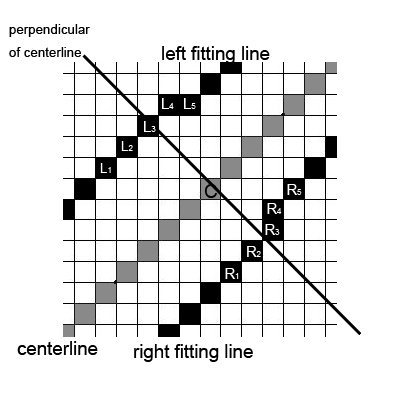
\includegraphics[width=3.0in]{line_fitting.png}\\
  \caption{Vessel Diameter Extraction}\label{fig:line_fitting}
\end{figure}

First, for specified centerline point $C(i,j)$ , we get two adjacent
neighbours on both its left and right side. Using this five points including
the point $C(i,j)$, we get the line $L_{c}$ crossing the centerline point.
Then we can achieve the perpendicular line's slope at point $C(i,j)$ and
compute its intersection point with the vascular structures contour $L_{3}$
and $R_{3}$. With these two points, we get the forward and backwards two
points of the contour. Then, we get the left intersection group $L=(L_{1},
L_{2}, L_{3}, L_{4}, L_{5})$ and the right $R=(R_{1}, R_{2}, R_{3}, R_{4},
R_{5})$ and the fitting lines $L_{l}$ and $L_{r}$ using the point groups. At
last, we obtain the intersection of $C_{L}(x_{l}, y_{l})$($L_{c}$ and
$L_{l}$) and $C_{R}(x_{r}, y_{r})$($L_{c}$ and $L_{r}$). We use the distance
$D=\sqrt{(x_{l}-x_{r})^2 + (y_{l}-y_{r})^2}$ as the vessel diameter at the
right position $C(i,j)$.

Using this method, we extract the diameters of Figure
\ref{fig:lineseg_trace},
%and the results are shown in Figure
%\ref{fig:diameter_extraction},
which are continuous and with slight
waving values.

%%\begin{figure}
%%  \centering
%%  % Requires \usepackage{graphicx}
%%  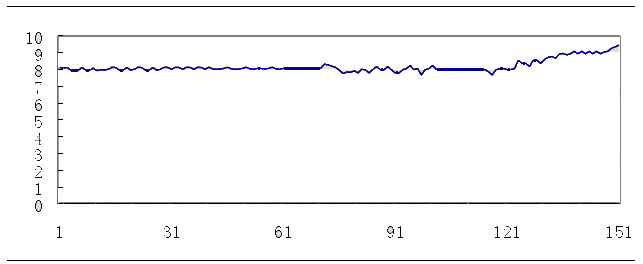
\includegraphics[width=3.0in]{diameter_extraction.png}\\
%%  \caption{Vessel Diameter Extraction Results}\label{fig:diameter_extraction}
%% \end{figure}


\subsection{3D Reconstruction of Coronary Arteries}
\subsubsection{Reconstruction Overview}

The angiograms is a procedure of projecting 3D objects to 2D
projection space during which many details may disappear and
foreshorten as well as overlapping. Just using the 2D projections to
justify the patient's conditions has inherent limitations. Using two
or several projections from multi views to reconstruct the topological
structures of the coronary arteries in 3D space is a useful method
during heart operations such as intervening.

The reconstruction of the coronary arteries are regarded to the type
of the X-Ray machines which can be divided into single-plane and
biplane machines. The reconstruction based on single-plane angiospasm
is to obtain several angles of views at the same moment of different
cardiac cycles, and uses these projections to reconstruct the vessels.
The difference between the biplane and the single-plane
reconstructions is biplane systems can achieve two synchronous
projection pairs at the same time without time error, leading to less
deformation of the vessels and high accuracy. For the reason that
biplane systems are much more expensive than single-planes and not common
in ordinary hospitals, we focus on the reconstruction of single-plane systems.

In order to reconstruct the 3D vessels, it is important to find the
corresponding points on each angiograms of different views for all 3D
points. In typical methods registration of the images between
different projection views are needed. However, there are problems
they are facing. No matter registrations based on features such as
bifurcations or any others, the first problem they are facing is that
the registration results are mostly not good enough even with many mistakes if
the changes among the views are large. The mistakes during
registration may lead to much more huge errors during the
reconstruction. The second problem is that these kinds of methods are
so fixed that neither constraints such as the connectivity of the
vessel neighbours nor some known conditions or knowledge can be added
which lead to a great waste of the various original information.

\subsubsection{Our Method}
The imaging modality of the X-Ray angiograms is different from the
ways other imaging devices such as cameras or vidicons work in. The
light source is the X-Ray source and the imaging plane is the
intensifier. The imaging procedure is mostly like perspective
projection under 3D space. We simulated this procedure using OpenGL.
This can be described in Figure \ref{fig:xray_work_way}

\begin{figure}
 \centering
  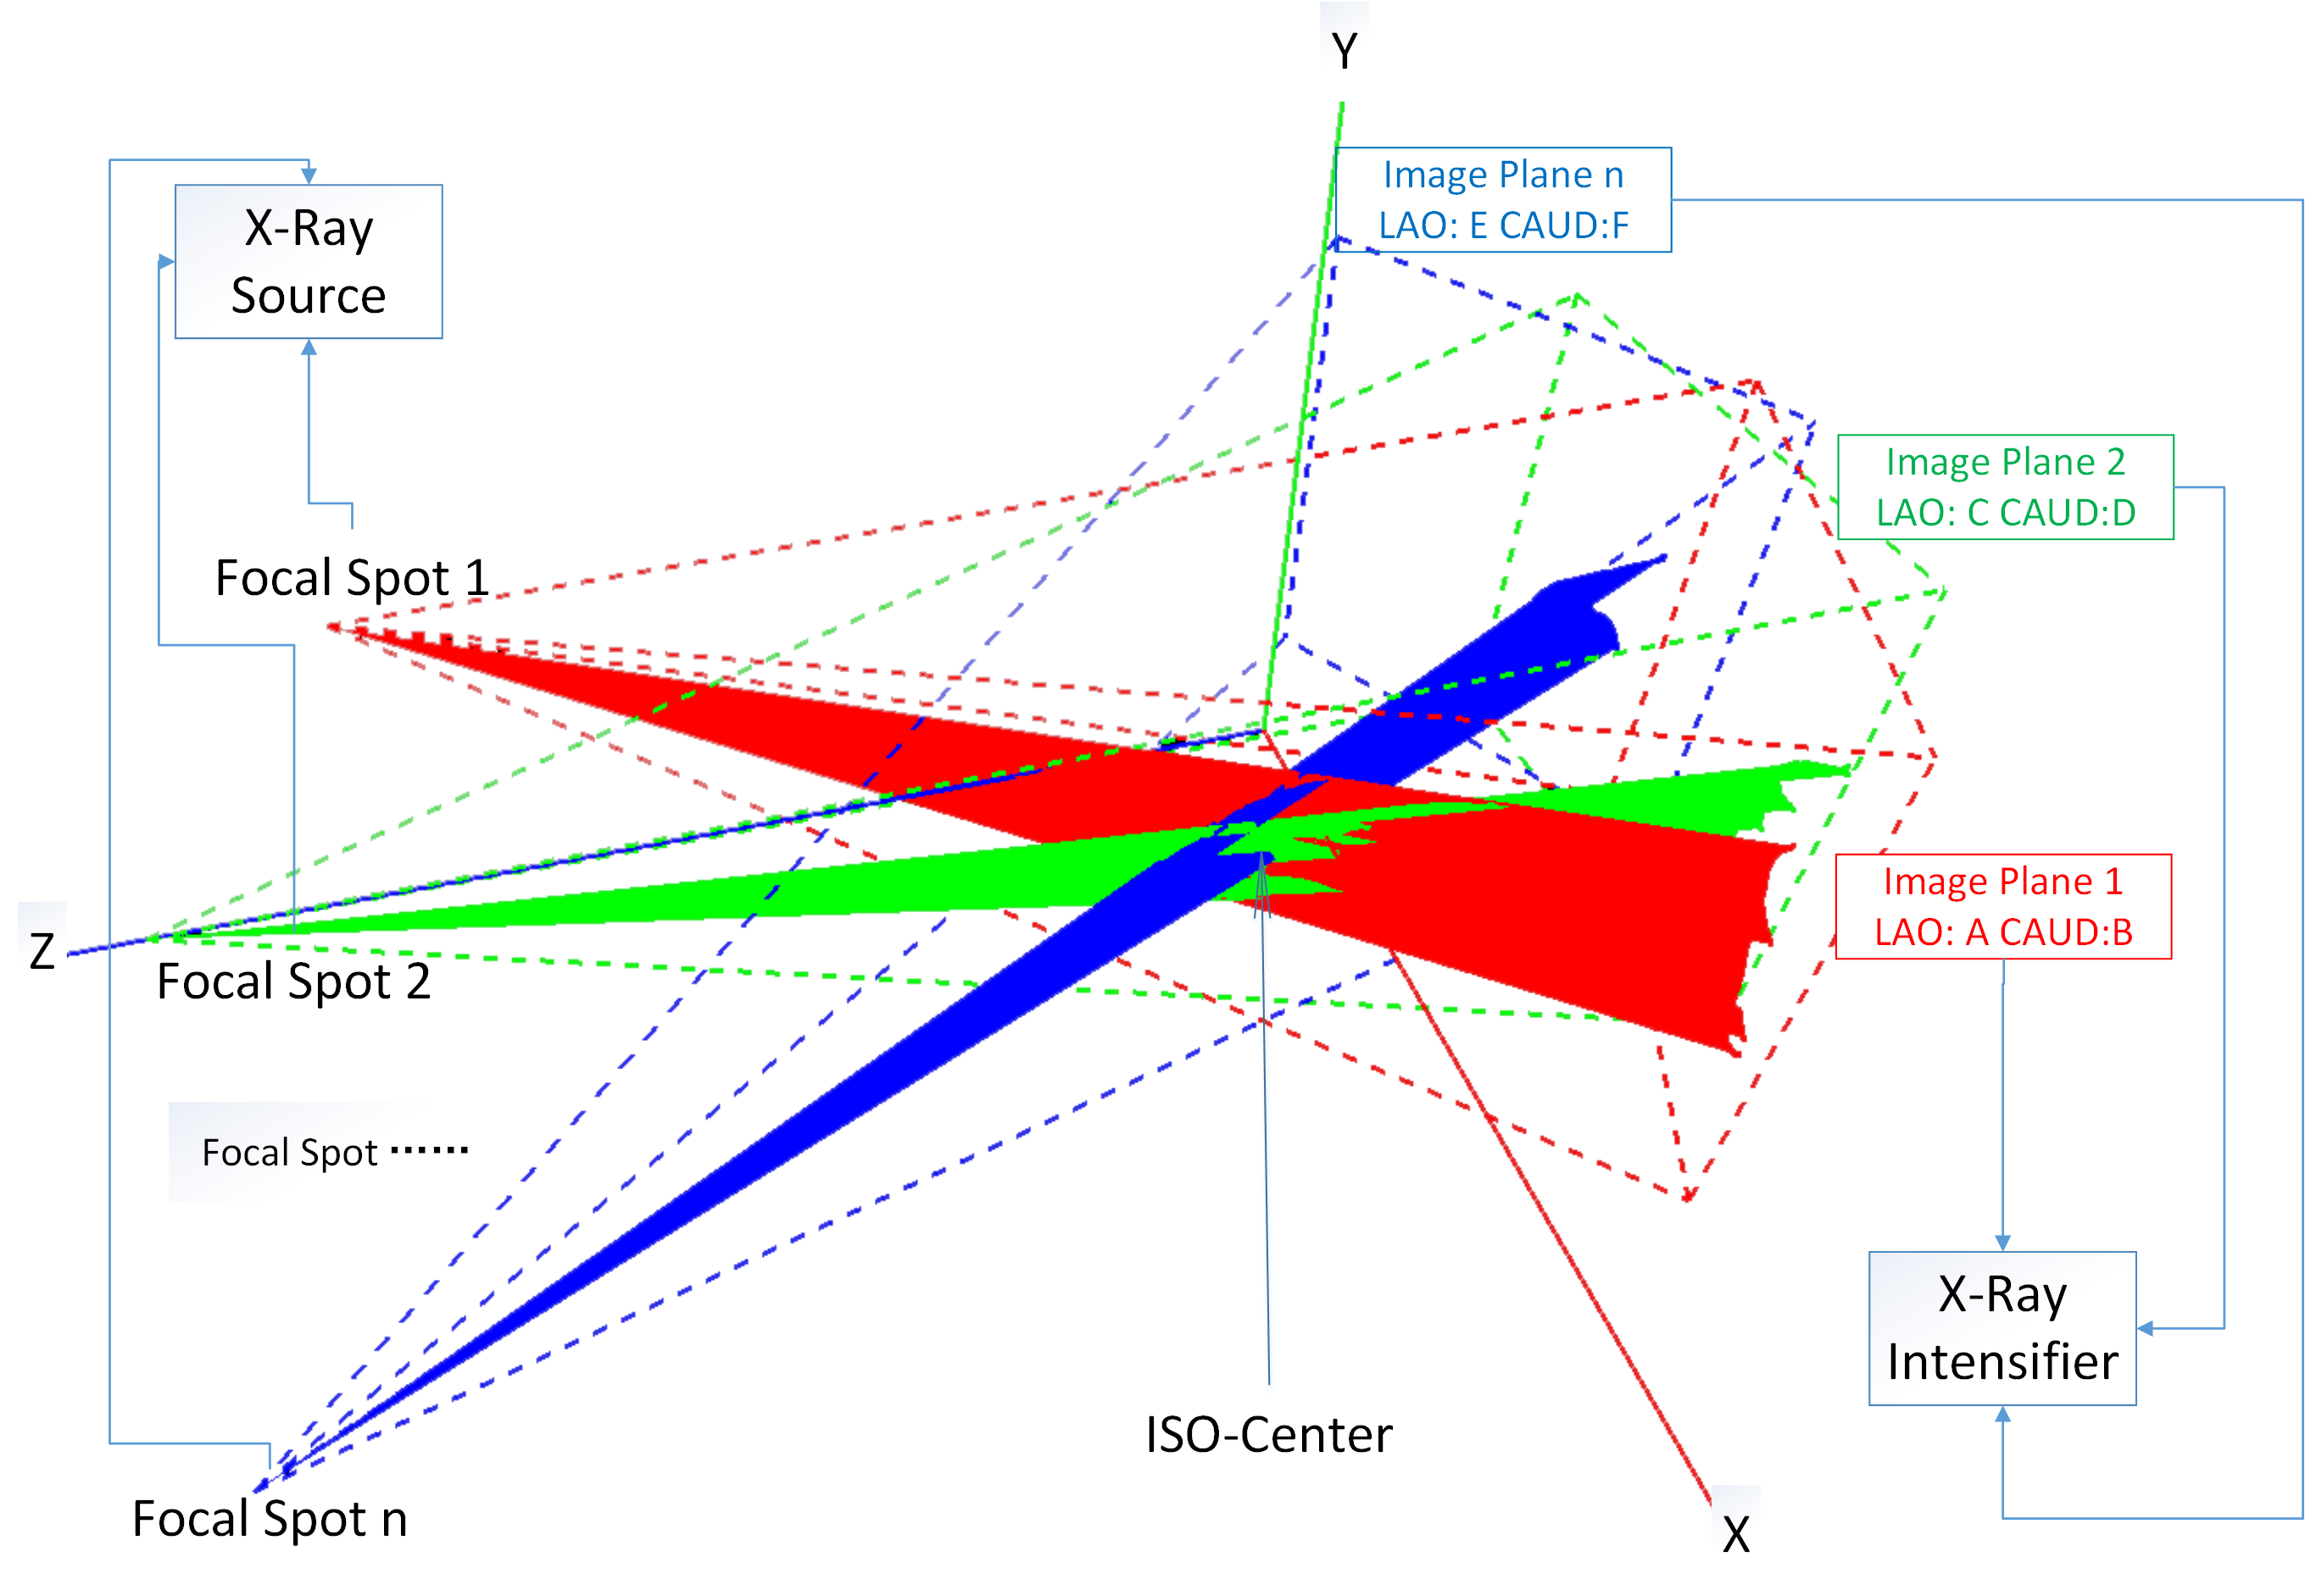
\includegraphics[width=3.0in]{x_ray_work.png}\\
  \caption{X-Ray Perspective Projection Of Vessel Skeletons}\label{fig:xray_work_way}
\end{figure}

The frustum of each color represents one view of the angiograms. The
source of the frustum could be seen as X-Ray source, while the far
plane could be seen as the intensifier. The vessel skeletons should be
at the iso-center. The exact intersected lines from every view should
be 3D space structures of the skeletons of the projected vessels.
Being aware of the diameters at every skeleton point, we can get the
structures of the vessels.

But the intersections are the correspondence between view pairs. The
computation of intersection lines (points) goes back to the
registration problem which are ill-posed. Also, due to precision and
other errors, it is hard to obtain the accurate intersections among
all the views.

However, on the other hand, the 3D skeletons could be regarded as
consisting of several skeleton segments. Each segment could be seen as
made up of sampled points. These points must be between the space of
the X-Ray source and the intensifier. Also, they should be mostly
projected onto every view.  So, if we sampled the space between source
and intensifier using a tiny enough uniform step, points or their
approximations that belong to the skeleton must be inside them.
Finally, the problem has transformed into how to extract these points.

In our opinion, each 3D point in the sampled space could be assigned
with a probability of being one of the 3D skeleton points. The
possibility could be determined by three main causes.
The first is how many views this point could be
projected onto. The second is the distance from the corresponding projected 2D
point on one view to the valid skeleton point on the same view.
Also, according to the continuity of the vascular structures,
the distance between neighbored points in the same skeleton should affect the possibility.

Finally, the sampled 3D space between the optical center and the
intensifier could be regarded as an Markov Random Field and the
reconstruction problem could be seen as an energy minimization problem
with consistent, continuous and topological constraints.

\subsubsection{Our Implementation}
In our approach, we use at least three views of angiograms at the same
cardiac cycle and choose the projection view $I_{1}$ as a reference
view which includes the least foreshortening and overlap among all the
views. The 3D space is divided into 3D slices which we call layer
$L=(l_{1}, l_{2}...l_{n})$ using a given depth increments which is
shown in Figure \ref{fig:c_arm_slices}.

\begin{figure}
  \centering
  % Requires \usepackage{graphicx}
  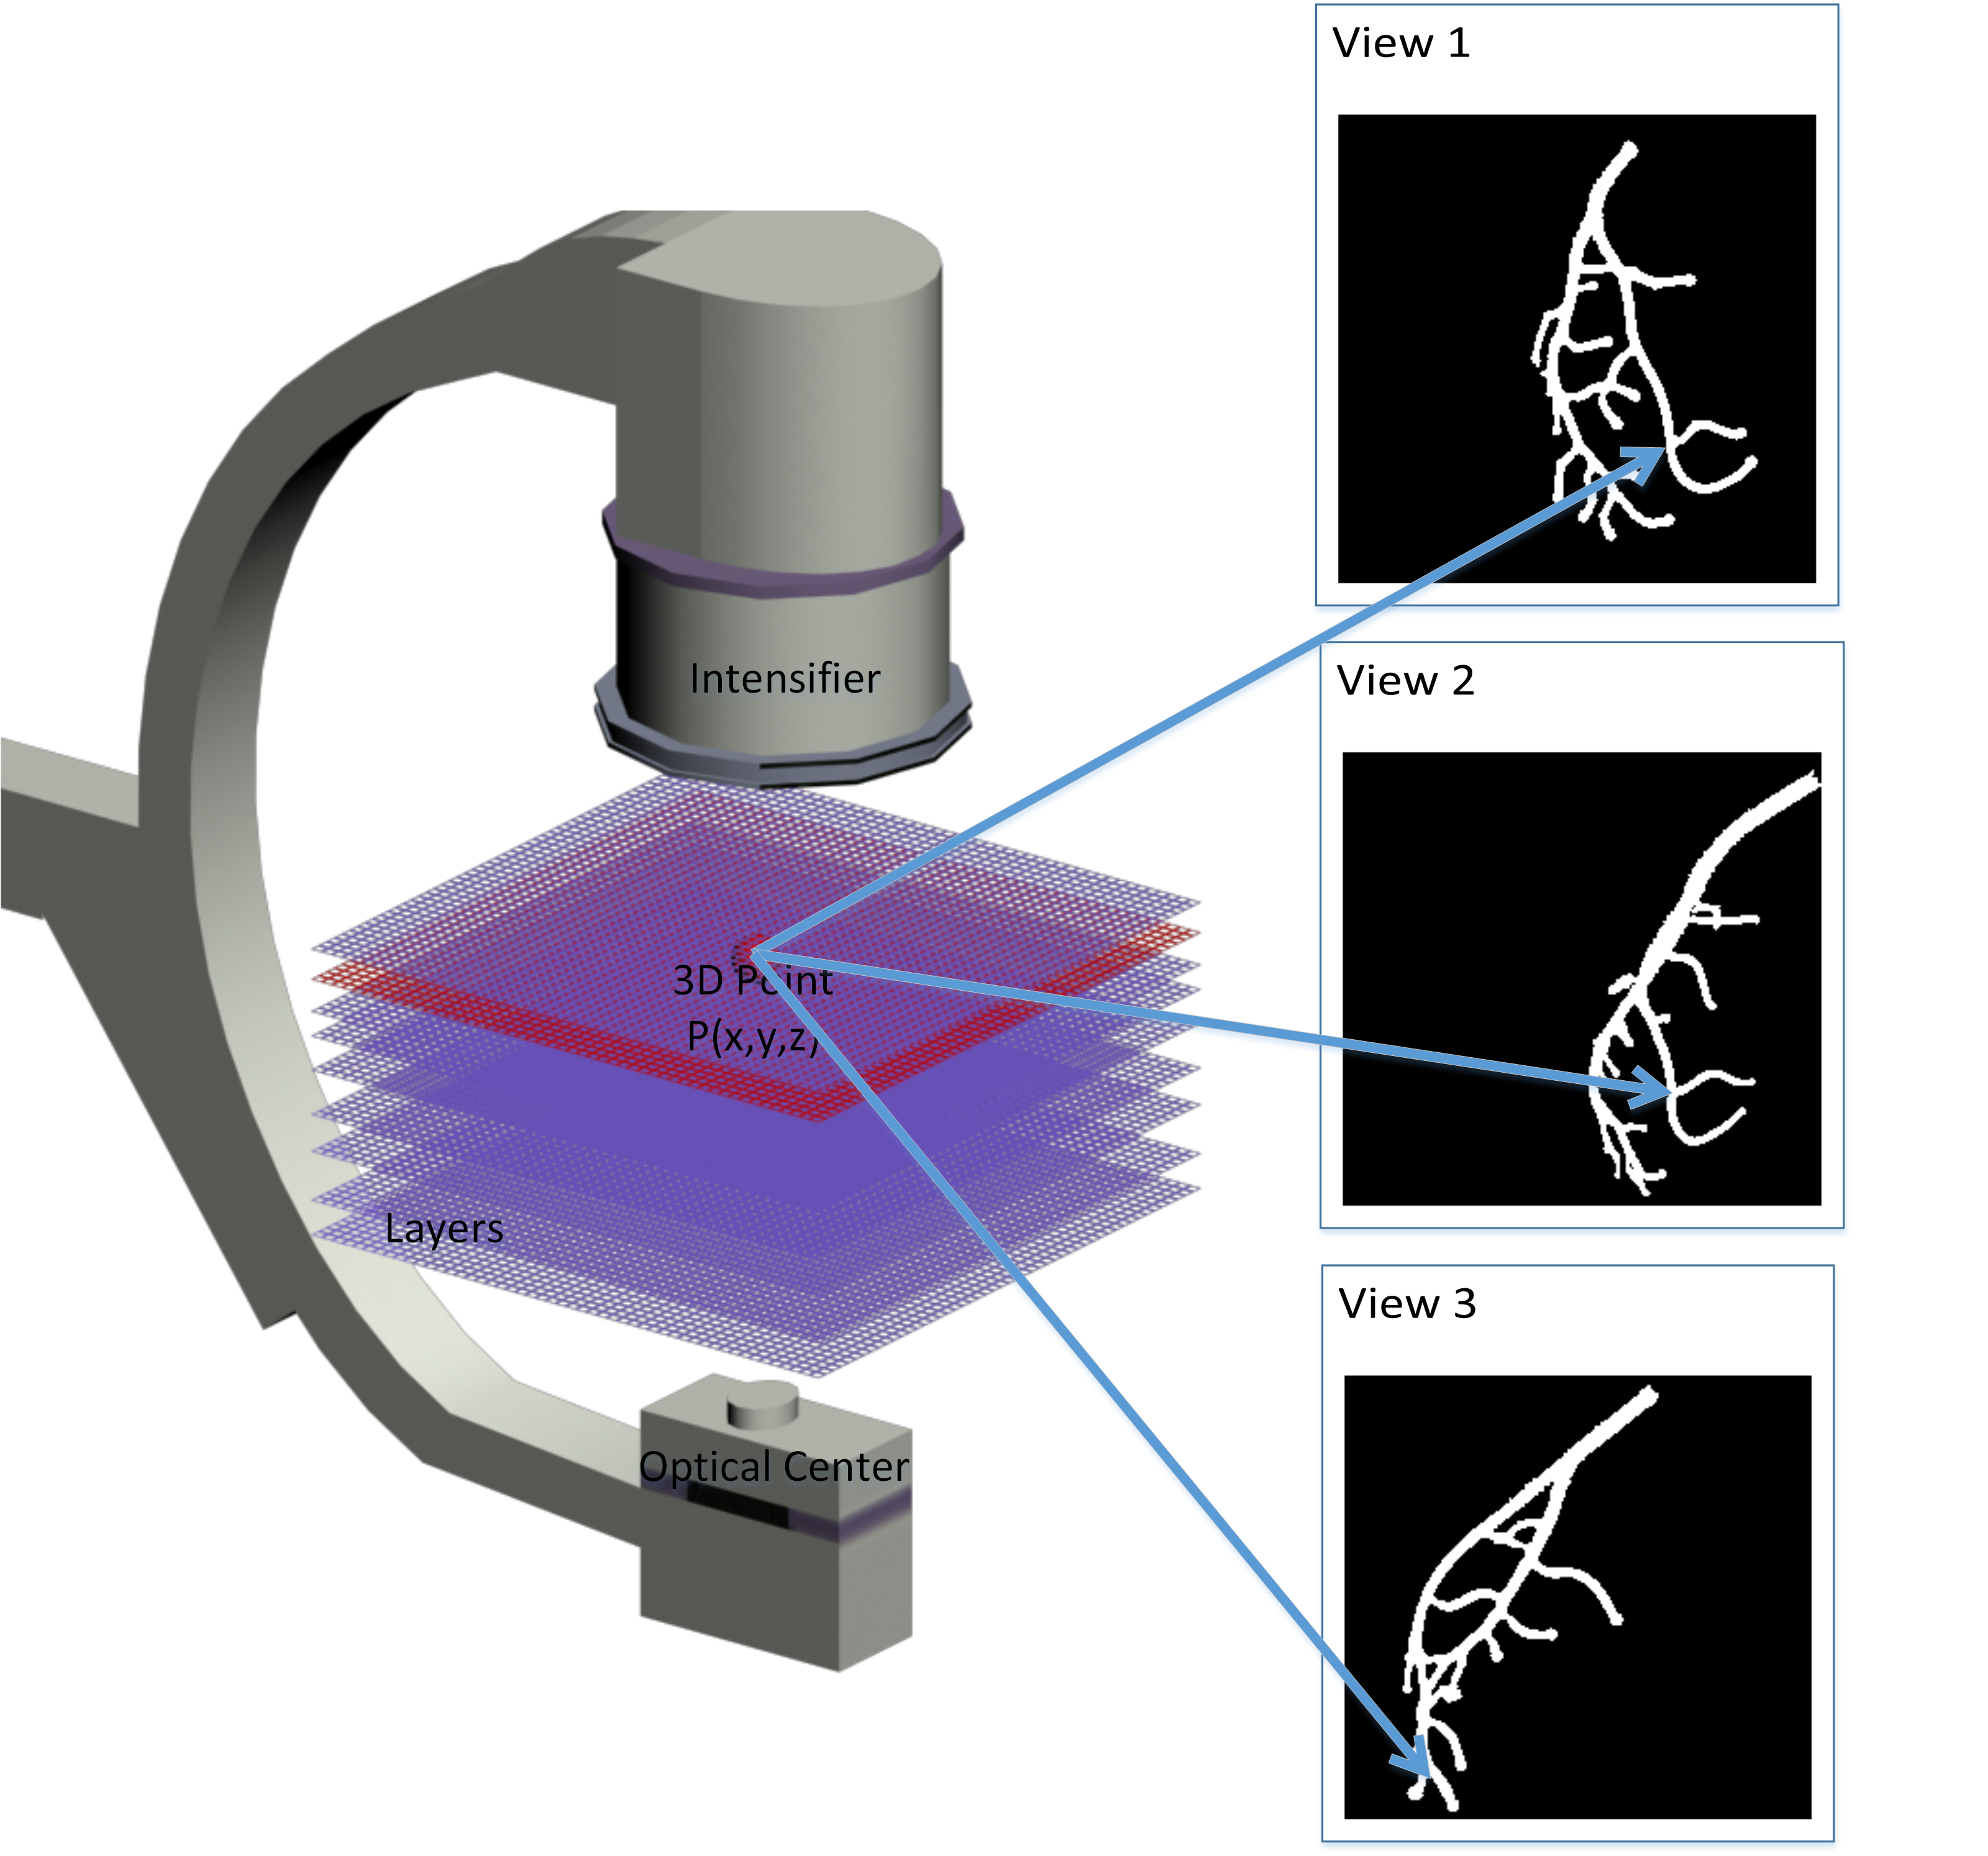
\includegraphics[width=3.0in]{c_arm_slices.png}\\
  \caption{3D Space Depth Slices}\label{fig:c_arm_slices}
\end{figure}

Each depth can be assigned with a label $l_{i}$. Meanwhile, each
skeleton point on reference view $I_{1}$ corresponds one projected
line from the source to the intensifier through all the layers.

Therefore, for a given pixel $p$ on $I_{1}$, the pair $(p,
l_{i})$ uniquely identifies a point in 3D space. So, the goal of the
3D reconstruction is to optimally assign an label $l_{i}$ to each $p$
on the centerline of the reference view $I_{1}$.  This problem can be
formulated as an energy minimization problem considering connectivity
and topological structures.The energy equation could be defined as

\begin{equation}
E(f) = \sum_{p\in P} D_{p}(f_{p}) + \lambda \sum_{p,q \in N} V_{p,q}(f_{p}, f_{q})
\end{equation}

Our goal is to find the minimum $E(f)$ and we use the belief propagation (BP)
method to achieve the solution.

In our method, we define the $V_{p,q}(f_{p}, f_{q})$ as the Euclidean
distance between point $p, q$. And we define the $D_{p}(f_{p})$ as the
\emph{color consistency} which can be described as

\begin{equation}
D_{p}(f_{p}) = \frac{1}{(n-1)} \sum_{i=2}^{n} P_{i}(x,y)
\end{equation}

where $P_{ith}(x,y)$ is the projection value of point $p$ on the
$ith$ view, which we define as

\begin{equation}
P_{ith}(x,y) =
\left\{
  \begin{array}{lll}
    W_{h}, & \hbox {$p(x,y) \in I_{ith}$} \\
    W_{l},  & \hbox {$\bigcup(p(x,y), 1) \notin I_{ith}$} \\
    W_{a}, & \hbox {else}
  \end{array}
\right.
\end{equation}

\begin{equation}
W_{a} = \frac{1}{N} \sum_{i=1}^{N} Val_{ith}(x,y)
\end{equation}

where $p(x,y)\in I_{ith}$ means that $p(x,y)$ is a valid centerline
point of $I_{ith}$, $W_{h}$ and $W_{l}$ are two constants that
control the very high and very low of the value. For a grey scale
image, $\bigcup(p(x,y), 1)$ is the 8 neighbors of the point
$p(x,y)$.  If $p(x,y)$ can not be found right in the $I_{ith}$, we
will compute its 8 neighbors and obtain the average value as the
value of point $p(x,y)$. And if none of its neighbors is valid, it
could be assigned with $ W_{l}$.

Our algorithm includes two main steps, message propagation and energy
minimization computation. In message propagation, the color value of
point $p(x,y) \in I_{1}$ is updated as

\begin{equation}
V_{p} = V_{p} + \alpha minD+ (1-\alpha)V_{p_{minD}})
\end{equation}

where $\alpha$ is a constant controlling the weight its neighbors'
\emph{color consistency} and \emph{dist consistency}. $minD$ stands for the minimum
distance from $p(x,y)$ to its neighbors. $V_{p_{minD}}$ stands for the
value of the minimum distance point.

In our energy minimization, different from typical BP, the current energy of the $ith$
depth($l_{i}$) is defined as

\begin{equation}
e_{i}(p_{i}) = min[\gamma D(p_{i}, q) + (1-\gamma)V(q) + e_{i-1}(q)];
\end{equation}

in which $q$ stands for the projected sample depths of
$\bigcup^\circ(p_{i}, 1)$ which is the neighbours of $p_{i}$ without including $p_{i}$
itself.

At last, we compute the minimum sum of all the grouped vessel skeletons' cost,
and obtain the optimal solution for the whole vessel skeleton tree.

After the reconstruction of the 3D skeletons of the coronary arteries,
using the diameters we extracted, we obtain the final result as shown in
Figure \ref{fig:final_result}.




\begin{figure}
  \centering
  % Requires \usepackage{graphicx}
  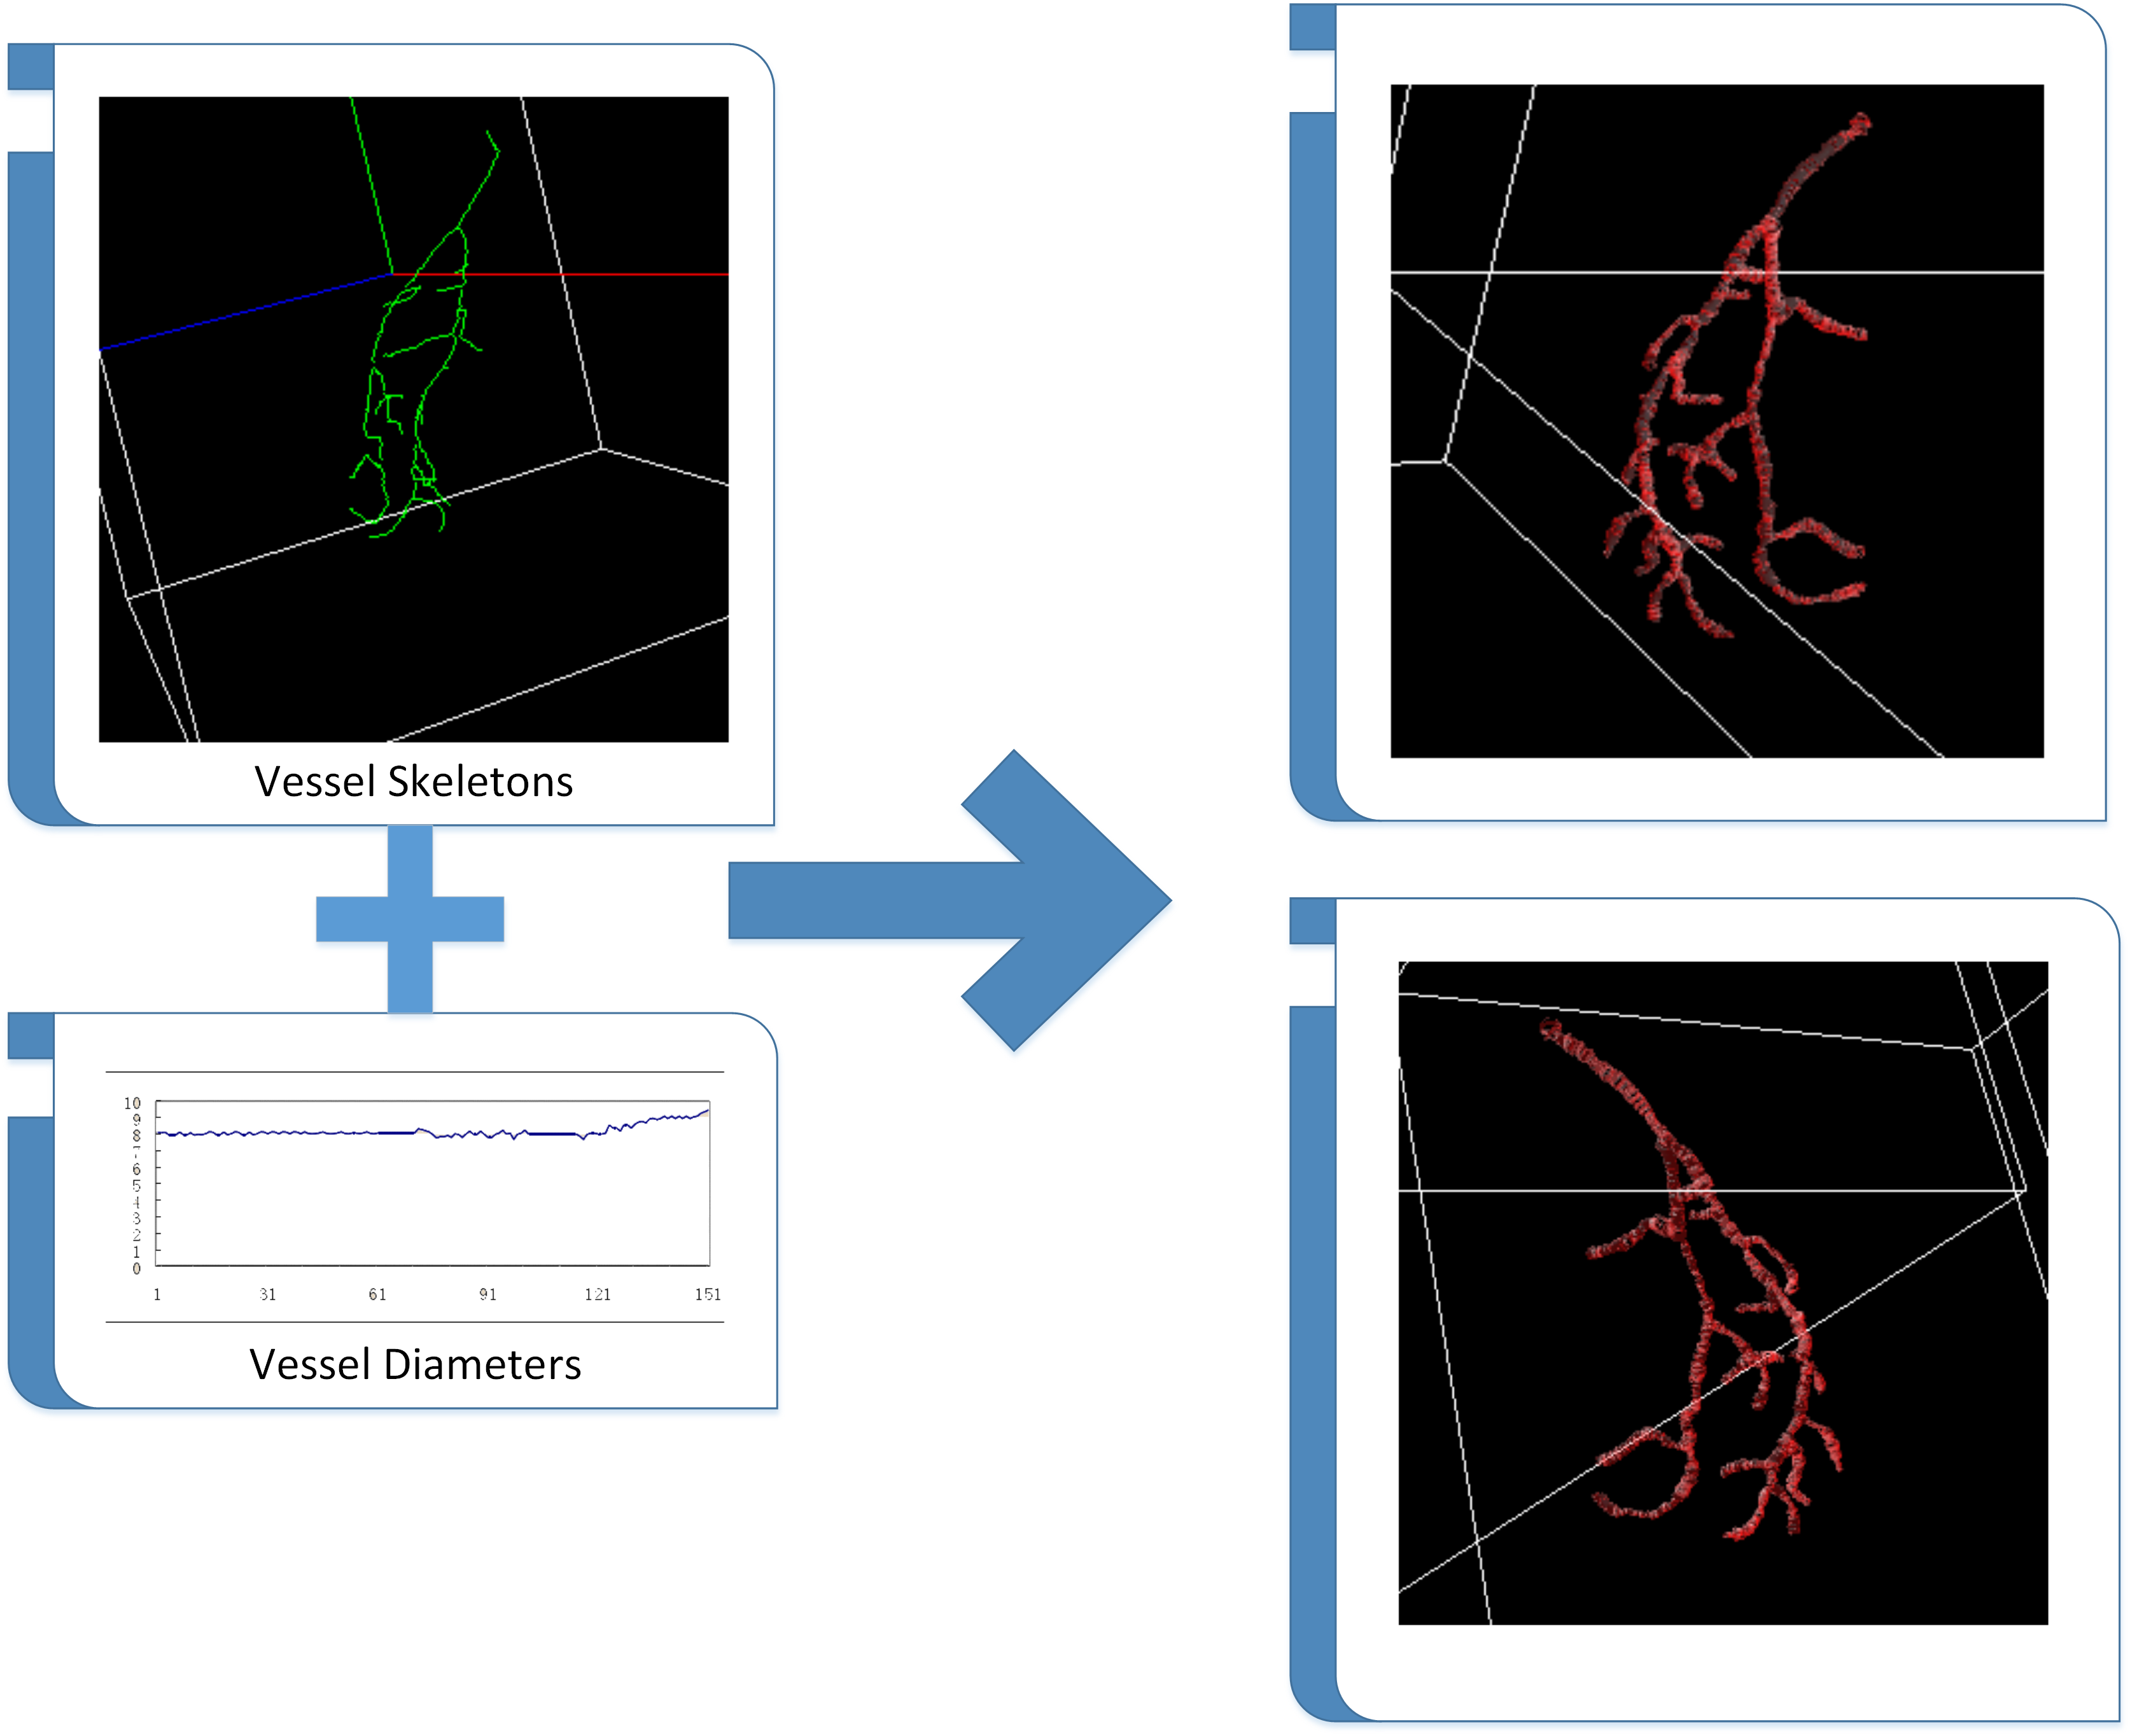
\includegraphics[width=3.0in]{final_result.png}
  \caption{The Skeleton with Diameters}
  \label{fig:final_result}
\end{figure}



\section{Experiments}\label{sec:experiments}
\subsection{Results}

The reconstruction method was experimented both on synthetical data and real
clinical data. Compared with real data, the reconstruction of synthetical
data is easy to assess because of knowing the vessel ground truth. The final
reconstruction results of synthetical data can be found in Figure
\ref{fig:experiments_full}.

\begin{figure*}
  \centering
  % Requires \usepackage{graphicx}
  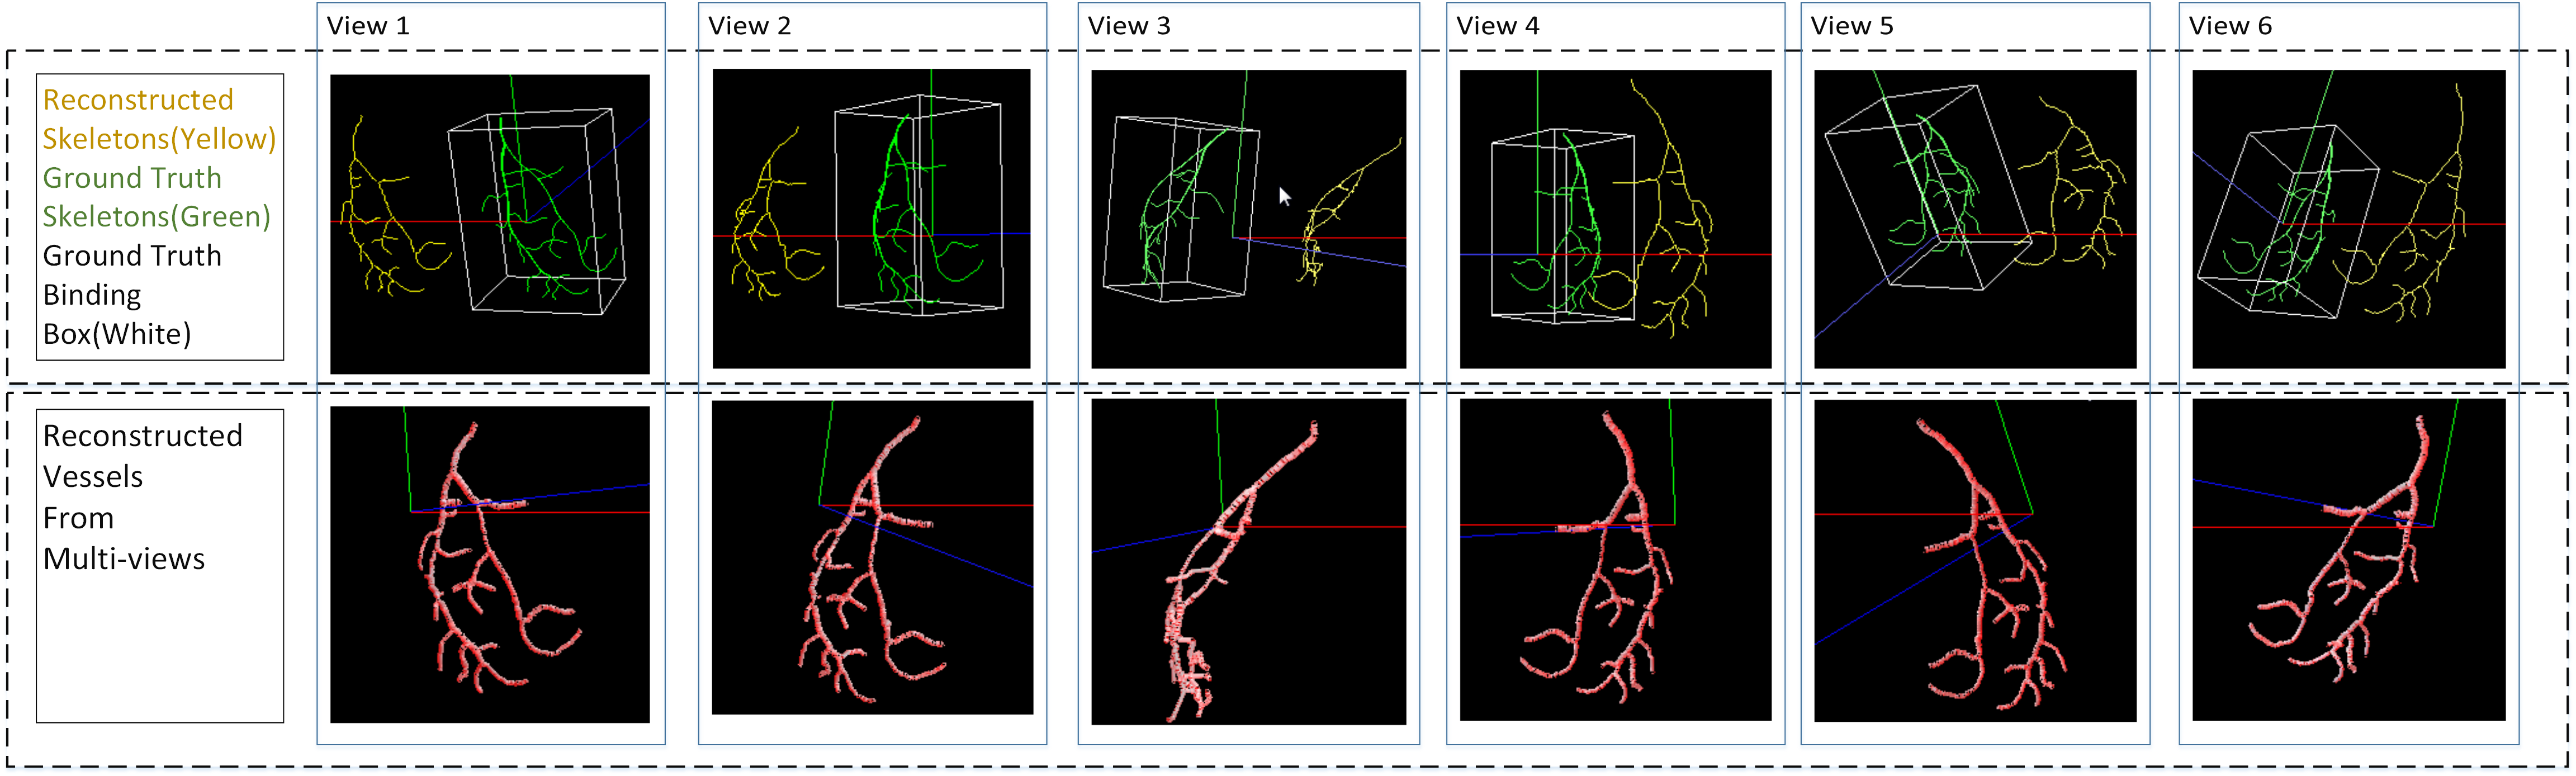
\includegraphics[width=6.0in]{experiments_full.png}\\
  \caption{Up: Reconstructed Centerlines and Ground Truth from Different Views; Down: Reconstructed Vessels}\label{fig:experiments_full}
\end{figure*}

In upper columns of Figure\ref{fig:experiments_full}, the yellow lines
indicate the reconstructed skeleton using our method. The green lines
indicate the ground truth obtained from our simulation platform. The white
box is the binding box of the ground truth. We use the size of the binding
box to evaluate the reconstructed skeletons. We compute the distance between
each ground truth point and the computed point.Then we compute the average
distance as the error. We use the scale the error divides the size of the
binding box to evaluate our reconstructed precision. The error statistics
are described as Figure \ref{fig:error_statistics}.

\begin{figure}
  \centering
  % Requires \usepackage{graphicx}
  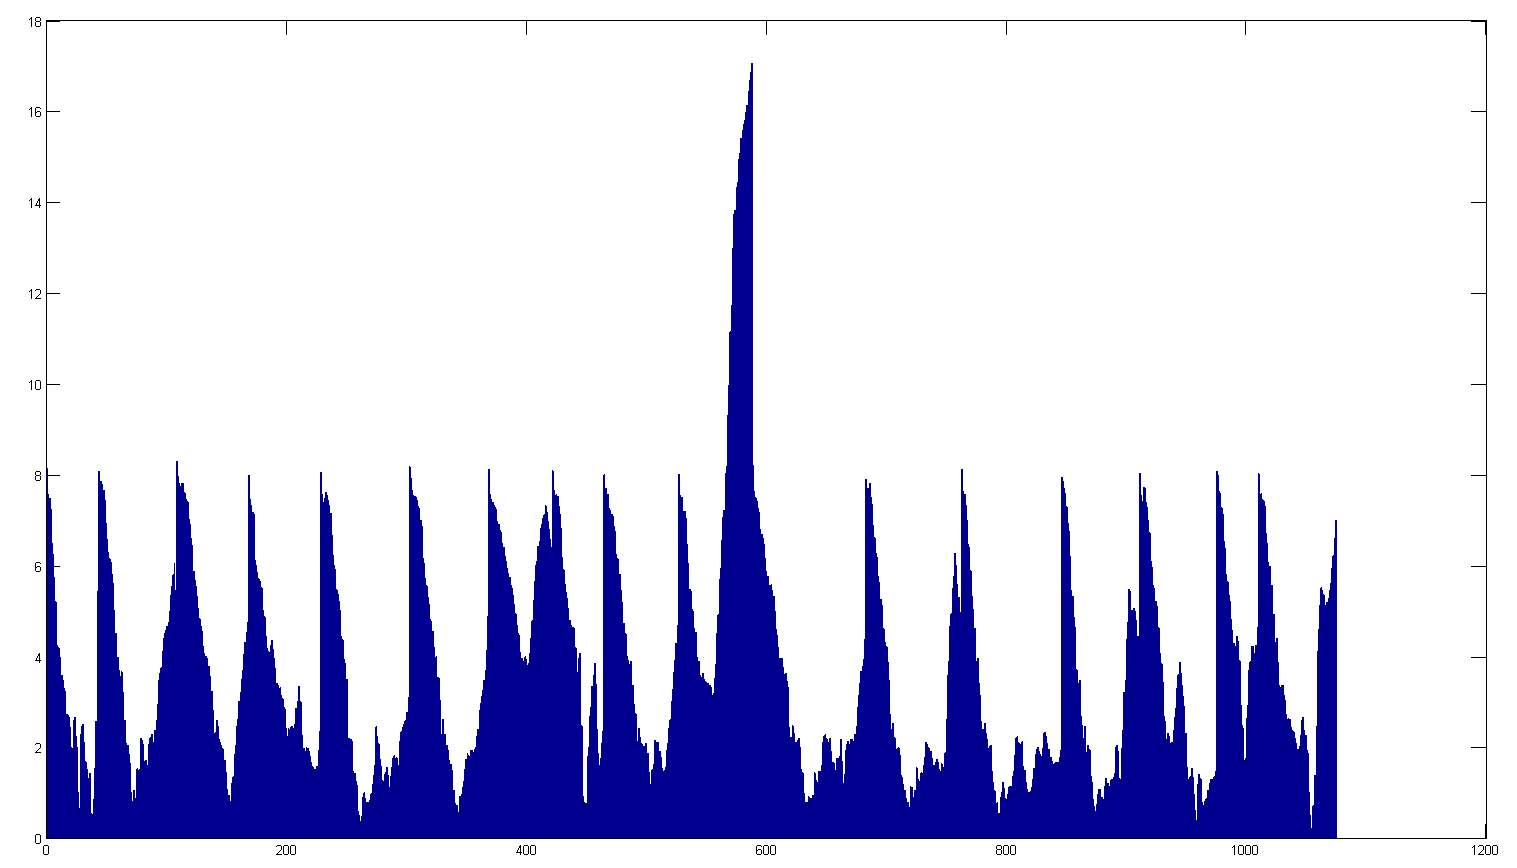
\includegraphics[width=3.0in]{error_statistics.png}\\
  \caption{Error Statistics between Reconstructed Skeletons and Ground Truth}\label{fig:error_statistics}
\end{figure}

Finally, we get an average error of 3.833708 and the binding box of
(52.691906, 77.026981, 39.552235).

As for the real data, the views and reconstructed data can be found in
Figure \ref{fig:real_reconstructed_data}.

\begin{figure}
  \centering
  % Requires \usepackage{graphicx}
  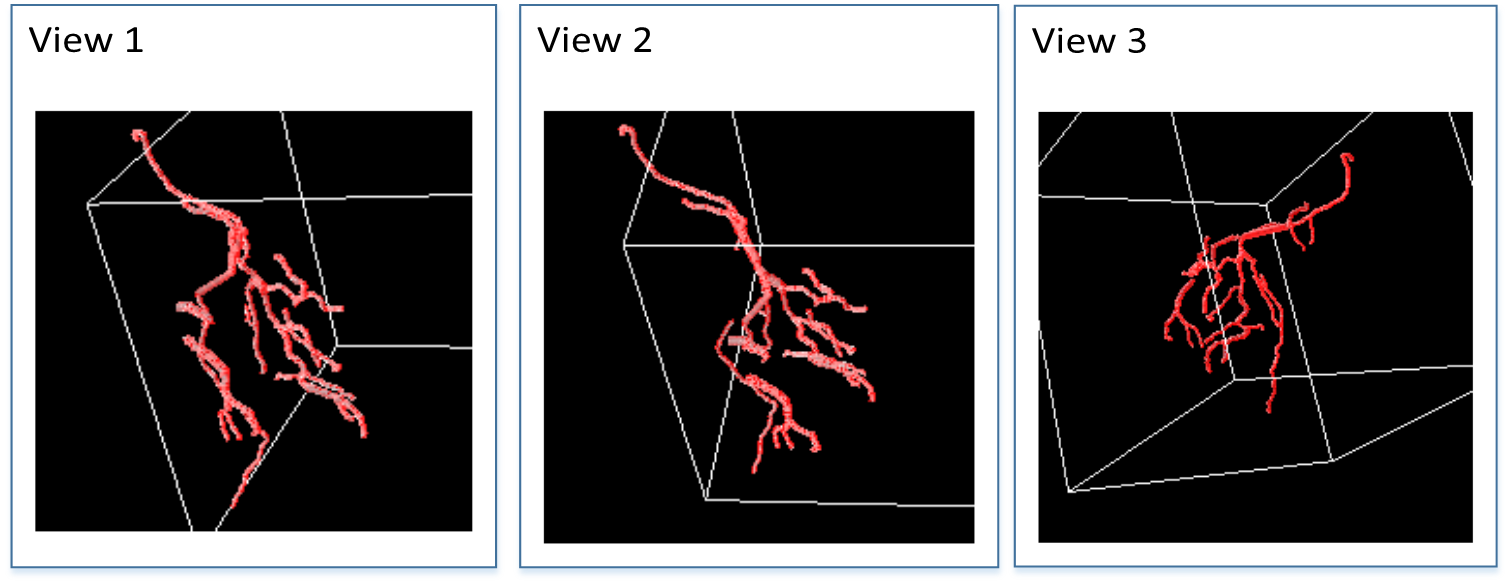
\includegraphics[width=3.0in]{real_data_final.png}\\
  \caption{Reconstructed Real Data}\label{fig:real_reconstructed_data}
\end{figure}

\subsection{Performance}
Our method consists of three steps and the consuming time of each step can
be described in Table \ref{tbl:performance}.

\begin{table}
\begin{tabular}{|c|c|c|c|}
\hline
Step &Called Times&Total Time&Average Time\\
\hline
1 & 57 & 66.024s & 1.158s \\
\hline
2 & 30 & 230.634s & 7.6878s \\
\hline
3 & 1 &27.3s & 27.3s \\
\hline
\end{tabular}
\caption{Step Execution Time}\label {tbl:performance}
\end{table}
Step 1 indicate Vessel Extraction, step 2 indicate Centerline Tracking and
step 3 indicate 3D Reconstruction. According to the table, the centerline
tracking and 3D reconstruction step consumes most time, in our future work,
we wanna implement them on GPU.


\section{Conclusion and Discussion}
\input{conclusion_discussion}

\section{Future Work}\label{sec:performance}
We use three projection views to reconstruct the coronary arteries. In our
current work, the corresponding image pairs are selected out by hand
according to the cardiac cycle. This can be accurate but slow down the
reconstruction speed. In the near future, we want to find some method to
find the corresponding images automatically. Also, our work is divided into
three main parts and the data processing consumes much time, we want to
accelerate the image processing step, as well as the reconstruction step
with the help of GPU. Finally, we want to build a real-time online
reconstruction system. 

%\begin{figure}[t]
%  \includegraphics[width=\linewidth]{test.eps}
%  \caption{Insert caption here.}
%\end{figure}

%% The Appendices part is started with the command \appendix;
%% appendix sections are then done as normal sections
%% \appendix

%% \section{}
%% \label{}

%% References
%%
%% Following citation commands can be used in the body text:
%% Usage of \cite is as follows:
%%   \cite{key}          ==>>  [#]
%%   \cite[chap. 2]{key} ==>>  [#, chap. 2]
%%   \citet{key}         ==>>  Author [#]
%% References with bibTeX database:
\bibliographystyle{elsarticle-num}
\bibliography{cadcg13_template}

%% Authors are advised to submit their bibtex database files. They are
%% requested to list a bibtex style file in the manuscript if they do
%% not want to use model3-num-names.bst.

%% References without bibTeX database:

% \begin{thebibliography}{00}

%% \bibitem must have the following form:
%%   \bibitem{key}...
%%

% \bibitem{}

% \end{thebibliography}


\end{document}

%%
%% End of file `cadcg13_template.tex'.
